\documentclass[twoside]{book}

% Packages required by doxygen
\usepackage{fixltx2e}
\usepackage{calc}
\usepackage{doxygen}
\usepackage[export]{adjustbox} % also loads graphicx
\usepackage{graphicx}
\usepackage[utf8]{inputenc}
\usepackage{makeidx}
\usepackage{multicol}
\usepackage{multirow}
\PassOptionsToPackage{warn}{textcomp}
\usepackage{textcomp}
\usepackage[nointegrals]{wasysym}
\usepackage[table]{xcolor}

% Font selection
\usepackage[T1]{fontenc}
\usepackage[scaled=.90]{helvet}
\usepackage{courier}
\usepackage{amssymb}
\usepackage{sectsty}
\renewcommand{\familydefault}{\sfdefault}
\allsectionsfont{%
  \fontseries{bc}\selectfont%
  \color{darkgray}%
}
\renewcommand{\DoxyLabelFont}{%
  \fontseries{bc}\selectfont%
  \color{darkgray}%
}
\newcommand{\+}{\discretionary{\mbox{\scriptsize$\hookleftarrow$}}{}{}}

% Page & text layout
\usepackage{geometry}
\geometry{%
  a4paper,%
  top=2.5cm,%
  bottom=2.5cm,%
  left=2.5cm,%
  right=2.5cm%
}
\tolerance=750
\hfuzz=15pt
\hbadness=750
\setlength{\emergencystretch}{15pt}
\setlength{\parindent}{0cm}
\setlength{\parskip}{3ex plus 2ex minus 2ex}
\makeatletter
\renewcommand{\paragraph}{%
  \@startsection{paragraph}{4}{0ex}{-1.0ex}{1.0ex}{%
    \normalfont\normalsize\bfseries\SS@parafont%
  }%
}
\renewcommand{\subparagraph}{%
  \@startsection{subparagraph}{5}{0ex}{-1.0ex}{1.0ex}{%
    \normalfont\normalsize\bfseries\SS@subparafont%
  }%
}
\makeatother

% Headers & footers
\usepackage{fancyhdr}
\pagestyle{fancyplain}
\fancyhead[LE]{\fancyplain{}{\bfseries\thepage}}
\fancyhead[CE]{\fancyplain{}{}}
\fancyhead[RE]{\fancyplain{}{\bfseries\leftmark}}
\fancyhead[LO]{\fancyplain{}{\bfseries\rightmark}}
\fancyhead[CO]{\fancyplain{}{}}
\fancyhead[RO]{\fancyplain{}{\bfseries\thepage}}
\fancyfoot[LE]{\fancyplain{}{}}
\fancyfoot[CE]{\fancyplain{}{}}
\fancyfoot[RE]{\fancyplain{}{\bfseries\scriptsize Generated by Doxygen }}
\fancyfoot[LO]{\fancyplain{}{\bfseries\scriptsize Generated by Doxygen }}
\fancyfoot[CO]{\fancyplain{}{}}
\fancyfoot[RO]{\fancyplain{}{}}
\renewcommand{\footrulewidth}{0.4pt}
\renewcommand{\chaptermark}[1]{%
  \markboth{#1}{}%
}
\renewcommand{\sectionmark}[1]{%
  \markright{\thesection\ #1}%
}

% Indices & bibliography
\usepackage{natbib}
\usepackage[titles]{tocloft}
\setcounter{tocdepth}{3}
\setcounter{secnumdepth}{5}
\makeindex

% Hyperlinks (required, but should be loaded last)
\usepackage{ifpdf}
\ifpdf
  \usepackage[pdftex,pagebackref=true]{hyperref}
\else
  \usepackage[ps2pdf,pagebackref=true]{hyperref}
\fi
\hypersetup{%
  colorlinks=true,%
  linkcolor=blue,%
  citecolor=blue,%
  unicode%
}

% Custom commands
\newcommand{\clearemptydoublepage}{%
  \newpage{\pagestyle{empty}\cleardoublepage}%
}

\usepackage{caption}
\captionsetup{labelsep=space,justification=centering,font={bf},singlelinecheck=off,skip=4pt,position=top}

%===== C O N T E N T S =====

\begin{document}

% Titlepage & ToC
\hypersetup{pageanchor=false,
             bookmarksnumbered=true,
             pdfencoding=unicode
            }
\pagenumbering{alph}
\begin{titlepage}
\vspace*{7cm}
\begin{center}%
{\Large homomorphine \\[1ex]\large .. }\\
\vspace*{1cm}
{\large Generated by Doxygen 1.8.13}\\
\end{center}
\end{titlepage}
\clearemptydoublepage
\pagenumbering{roman}
\tableofcontents
\clearemptydoublepage
\pagenumbering{arabic}
\hypersetup{pageanchor=true}

%--- Begin generated contents ---
\chapter{Hierarchical Index}
\section{Class Hierarchy}
This inheritance list is sorted roughly, but not completely, alphabetically\+:\begin{DoxyCompactList}
\item \contentsline{section}{homomorphine\+::Api}{\pageref{classhomomorphine_1_1_api}}{}
\item \contentsline{section}{homomorphine\+::Api\+Response}{\pageref{classhomomorphine_1_1_api_response}}{}
\item \contentsline{section}{homomorphine\+::Arithmetic\+Backend\+Factory}{\pageref{classhomomorphine_1_1_arithmetic_backend_factory}}{}
\item \contentsline{section}{homomorphine\+::Backend}{\pageref{classhomomorphine_1_1_backend}}{}
\begin{DoxyCompactList}
\item \contentsline{section}{homomorphine\+::Arithmetic\+Backend}{\pageref{classhomomorphine_1_1_arithmetic_backend}}{}
\begin{DoxyCompactList}
\item \contentsline{section}{homomorphine\+::H\+E\+Lib\+Backend}{\pageref{classhomomorphine_1_1_h_e_lib_backend}}{}
\item \contentsline{section}{homomorphine\+::Seal\+Backend}{\pageref{classhomomorphine_1_1_seal_backend}}{}
\item \contentsline{section}{homomorphine\+::T\+F\+H\+E\+Backend}{\pageref{classhomomorphine_1_1_t_f_h_e_backend}}{}
\end{DoxyCompactList}
\item \contentsline{section}{homomorphine\+::Arithmetic\+Backend}{\pageref{classhomomorphine_1_1_arithmetic_backend}}{}
\end{DoxyCompactList}
\item \contentsline{section}{homomorphine\+::Config}{\pageref{classhomomorphine_1_1_config}}{}
\item \contentsline{section}{homomorphine\+::Constants}{\pageref{classhomomorphine_1_1_constants}}{}
\item exception\begin{DoxyCompactList}
\item \contentsline{section}{homomorphine\+::Backend\+Exception}{\pageref{classhomomorphine_1_1_backend_exception}}{}
\item \contentsline{section}{homomorphine\+::Backend\+Factory\+Exception}{\pageref{classhomomorphine_1_1_backend_factory_exception}}{}
\item \contentsline{section}{homomorphine\+::Backend\+Operation\+Not\+Supported}{\pageref{classhomomorphine_1_1_backend_operation_not_supported}}{}
\end{DoxyCompactList}
\item \contentsline{section}{homomorphine\+::Interface}{\pageref{classhomomorphine_1_1_interface}}{}
\item \contentsline{section}{long\+\_\+array\+\_\+t}{\pageref{structlong__array__t}}{}
\item \contentsline{section}{homomorphine\+::Server}{\pageref{classhomomorphine_1_1_server}}{}
\item \contentsline{section}{homomorphine\+::Util}{\pageref{classhomomorphine_1_1_util}}{}
\end{DoxyCompactList}

\chapter{Class Index}
\section{Class List}
Here are the classes, structs, unions and interfaces with brief descriptions\+:\begin{DoxyCompactList}
\item\contentsline{section}{\mbox{\hyperlink{classhomomorphine_1_1_api}{homomorphine\+::\+Api}} }{\pageref{classhomomorphine_1_1_api}}{}
\item\contentsline{section}{\mbox{\hyperlink{classhomomorphine_1_1_api_response}{homomorphine\+::\+Api\+Response}} }{\pageref{classhomomorphine_1_1_api_response}}{}
\item\contentsline{section}{\mbox{\hyperlink{classhomomorphine_1_1_arithmetic_backend}{homomorphine\+::\+Arithmetic\+Backend}} }{\pageref{classhomomorphine_1_1_arithmetic_backend}}{}
\item\contentsline{section}{\mbox{\hyperlink{classhomomorphine_1_1_arithmetic_backend_factory}{homomorphine\+::\+Arithmetic\+Backend\+Factory}} }{\pageref{classhomomorphine_1_1_arithmetic_backend_factory}}{}
\item\contentsline{section}{\mbox{\hyperlink{classhomomorphine_1_1_arithmetic_backend_factory_exception}{homomorphine\+::\+Arithmetic\+Backend\+Factory\+Exception}} }{\pageref{classhomomorphine_1_1_arithmetic_backend_factory_exception}}{}
\item\contentsline{section}{\mbox{\hyperlink{classhomomorphine_1_1_backend}{homomorphine\+::\+Backend}} }{\pageref{classhomomorphine_1_1_backend}}{}
\item\contentsline{section}{\mbox{\hyperlink{classhomomorphine_1_1_backend_exception}{homomorphine\+::\+Backend\+Exception}} }{\pageref{classhomomorphine_1_1_backend_exception}}{}
\item\contentsline{section}{\mbox{\hyperlink{classhomomorphine_1_1_backend_operation_not_supported}{homomorphine\+::\+Backend\+Operation\+Not\+Supported}} }{\pageref{classhomomorphine_1_1_backend_operation_not_supported}}{}
\item\contentsline{section}{\mbox{\hyperlink{structblob__t}{blob\+\_\+t}} \\*Wrapper around the char/byte array }{\pageref{structblob__t}}{}
\item\contentsline{section}{\mbox{\hyperlink{classhomomorphine_1_1_boolean_circuit_backend}{homomorphine\+::\+Boolean\+Circuit\+Backend}} }{\pageref{classhomomorphine_1_1_boolean_circuit_backend}}{}
\item\contentsline{section}{\mbox{\hyperlink{classhomomorphine_1_1_boolean_circuit_backend_factory}{homomorphine\+::\+Boolean\+Circuit\+Backend\+Factory}} }{\pageref{classhomomorphine_1_1_boolean_circuit_backend_factory}}{}
\item\contentsline{section}{\mbox{\hyperlink{classhomomorphine_1_1_boolean_circuit_backend_factory_exception}{homomorphine\+::\+Boolean\+Circuit\+Backend\+Factory\+Exception}} }{\pageref{classhomomorphine_1_1_boolean_circuit_backend_factory_exception}}{}
\item\contentsline{section}{\mbox{\hyperlink{classhomomorphine_1_1_config}{homomorphine\+::\+Config}} }{\pageref{classhomomorphine_1_1_config}}{}
\item\contentsline{section}{\mbox{\hyperlink{classhomomorphine_1_1_constants}{homomorphine\+::\+Constants}} }{\pageref{classhomomorphine_1_1_constants}}{}
\item\contentsline{section}{\mbox{\hyperlink{classhomomorphine_1_1_h_e_lib_backend}{homomorphine\+::\+H\+E\+Lib\+Backend}} }{\pageref{classhomomorphine_1_1_h_e_lib_backend}}{}
\item\contentsline{section}{\mbox{\hyperlink{classhomomorphine_1_1_interface}{homomorphine\+::\+Interface}} }{\pageref{classhomomorphine_1_1_interface}}{}
\item\contentsline{section}{\mbox{\hyperlink{structlong__array__t}{long\+\_\+array\+\_\+t}} \\*Wrapper around the array, or vector of values }{\pageref{structlong__array__t}}{}
\item\contentsline{section}{\mbox{\hyperlink{classhomomorphine_1_1_seal_backend}{homomorphine\+::\+Seal\+Backend}} }{\pageref{classhomomorphine_1_1_seal_backend}}{}
\item\contentsline{section}{\mbox{\hyperlink{classhomomorphine_1_1_server}{homomorphine\+::\+Server}} }{\pageref{classhomomorphine_1_1_server}}{}
\item\contentsline{section}{\mbox{\hyperlink{classhomomorphine_1_1_t_f_h_e_backend}{homomorphine\+::\+T\+F\+H\+E\+Backend}} }{\pageref{classhomomorphine_1_1_t_f_h_e_backend}}{}
\item\contentsline{section}{\mbox{\hyperlink{classhomomorphine_1_1_util}{homomorphine\+::\+Util}} }{\pageref{classhomomorphine_1_1_util}}{}
\end{DoxyCompactList}

\chapter{Class Documentation}
\hypertarget{classhomomorphine_1_1_api}{}\section{homomorphine\+::Api Class Reference}
\label{classhomomorphine_1_1_api}\index{homomorphine::Api@{homomorphine::Api}}


{\ttfamily \#include $<$api.\+hpp$>$}

\subsection*{Public Member Functions}
\begin{DoxyCompactItemize}
\item 
\mbox{\hyperlink{classhomomorphine_1_1_api_response}{Api\+Response}} \mbox{\hyperlink{classhomomorphine_1_1_api_aa595d352d3494870f5e5bd7262be90c2}{get}} (vector$<$ string $>$ \&path)
\item 
\mbox{\hyperlink{classhomomorphine_1_1_api_response}{Api\+Response}} \mbox{\hyperlink{classhomomorphine_1_1_api_ab538a352f9ef7e92885bdd25a2f3dedd}{post}} (vector$<$ string $>$ \&path, string body)
\end{DoxyCompactItemize}


\subsection{Detailed Description}
/brief Provides a R\+E\+S\+T\+Ful A\+PI interface.

This class provides a R\+E\+S\+T\+Ful A\+PI interface for Homomorphine, it is very simple and does not expose a full functionality of Homomorphine, but rather selected group of functionalities. It is not advised to use this interface except for testing Homomorphine functionalities (R\+E\+S\+T\+Ful interface will be provided by the Golang wrapper around Homomorphine). 

\subsection{Member Function Documentation}
\mbox{\Hypertarget{classhomomorphine_1_1_api_aa595d352d3494870f5e5bd7262be90c2}\label{classhomomorphine_1_1_api_aa595d352d3494870f5e5bd7262be90c2}} 
\index{homomorphine::Api@{homomorphine::Api}!get@{get}}
\index{get@{get}!homomorphine::Api@{homomorphine::Api}}
\subsubsection{\texorpdfstring{get()}{get()}}
{\footnotesize\ttfamily \mbox{\hyperlink{classhomomorphine_1_1_api_response}{Api\+Response}} homomorphine\+::\+Api\+::get (\begin{DoxyParamCaption}\item[{vector$<$ string $>$ \&}]{path }\end{DoxyParamCaption})}

Handler for processing G\+ET H\+T\+TP requests.


\begin{DoxyParams}{Parameters}
{\em path} & full path of the H\+T\+TP request \\
\hline
\end{DoxyParams}
\begin{DoxyReturn}{Returns}
A\+PI response 
\end{DoxyReturn}
\mbox{\Hypertarget{classhomomorphine_1_1_api_ab538a352f9ef7e92885bdd25a2f3dedd}\label{classhomomorphine_1_1_api_ab538a352f9ef7e92885bdd25a2f3dedd}} 
\index{homomorphine::Api@{homomorphine::Api}!post@{post}}
\index{post@{post}!homomorphine::Api@{homomorphine::Api}}
\subsubsection{\texorpdfstring{post()}{post()}}
{\footnotesize\ttfamily \mbox{\hyperlink{classhomomorphine_1_1_api_response}{Api\+Response}} homomorphine\+::\+Api\+::post (\begin{DoxyParamCaption}\item[{vector$<$ string $>$ \&}]{path,  }\item[{string}]{body }\end{DoxyParamCaption})}

Handler for processing P\+O\+ST H\+T\+TP requests.


\begin{DoxyParams}{Parameters}
{\em path} & full path of the H\+T\+TP request \\
\hline
{\em body} & content of the body of H\+T\+TP requrest \\
\hline
\end{DoxyParams}
\begin{DoxyReturn}{Returns}
A\+PI response 
\end{DoxyReturn}


The documentation for this class was generated from the following files\+:\begin{DoxyCompactItemize}
\item 
src/api.\+hpp\item 
src/api.\+cpp\end{DoxyCompactItemize}

\hypertarget{classhomomorphine_1_1_api_response}{}\section{homomorphine\+::Api\+Response Class Reference}
\label{classhomomorphine_1_1_api_response}\index{homomorphine::ApiResponse@{homomorphine::ApiResponse}}


{\ttfamily \#include $<$api.\+hpp$>$}

\subsection*{Public Member Functions}
\begin{DoxyCompactItemize}
\item 
status\+\_\+code \mbox{\hyperlink{classhomomorphine_1_1_api_response_abe5d8dbece3cffee08905bb9389a8fd0}{get\+Status}} ()
\item 
void \mbox{\hyperlink{classhomomorphine_1_1_api_response_a3823ad464f6011397be80c62e391171c}{set\+Status}} (status\+\_\+code status)
\item 
json\+::value \mbox{\hyperlink{classhomomorphine_1_1_api_response_ae816a0c652d2cd47d88a67dda85024c4}{get\+Content}} ()
\item 
void \mbox{\hyperlink{classhomomorphine_1_1_api_response_aee304405cacc0b976145d2a3465ea7e5}{set\+Content}} (json\+::value \&content)
\end{DoxyCompactItemize}


\subsection{Detailed Description}
/brief R\+E\+S\+T\+Ful A\+PI response.

Simple A\+PI response wrapper used by Homomorphine R\+E\+S\+T\+Ful A\+PI 

\subsection{Member Function Documentation}
\mbox{\Hypertarget{classhomomorphine_1_1_api_response_ae816a0c652d2cd47d88a67dda85024c4}\label{classhomomorphine_1_1_api_response_ae816a0c652d2cd47d88a67dda85024c4}} 
\index{homomorphine::ApiResponse@{homomorphine::ApiResponse}!getContent@{getContent}}
\index{getContent@{getContent}!homomorphine::ApiResponse@{homomorphine::ApiResponse}}
\subsubsection{\texorpdfstring{getContent()}{getContent()}}
{\footnotesize\ttfamily json\+::value homomorphine\+::\+Api\+Response\+::get\+Content (\begin{DoxyParamCaption}{ }\end{DoxyParamCaption})}

Returns the full J\+S\+ON content of the A\+PI response .

\begin{DoxyReturn}{Returns}
J\+S\+ON object of A\+PI response 
\end{DoxyReturn}
\mbox{\Hypertarget{classhomomorphine_1_1_api_response_abe5d8dbece3cffee08905bb9389a8fd0}\label{classhomomorphine_1_1_api_response_abe5d8dbece3cffee08905bb9389a8fd0}} 
\index{homomorphine::ApiResponse@{homomorphine::ApiResponse}!getStatus@{getStatus}}
\index{getStatus@{getStatus}!homomorphine::ApiResponse@{homomorphine::ApiResponse}}
\subsubsection{\texorpdfstring{getStatus()}{getStatus()}}
{\footnotesize\ttfamily status\+\_\+code homomorphine\+::\+Api\+Response\+::get\+Status (\begin{DoxyParamCaption}{ }\end{DoxyParamCaption})}

Returns the status of the response.

\begin{DoxyReturn}{Returns}
response status code 
\end{DoxyReturn}
\mbox{\Hypertarget{classhomomorphine_1_1_api_response_aee304405cacc0b976145d2a3465ea7e5}\label{classhomomorphine_1_1_api_response_aee304405cacc0b976145d2a3465ea7e5}} 
\index{homomorphine::ApiResponse@{homomorphine::ApiResponse}!setContent@{setContent}}
\index{setContent@{setContent}!homomorphine::ApiResponse@{homomorphine::ApiResponse}}
\subsubsection{\texorpdfstring{setContent()}{setContent()}}
{\footnotesize\ttfamily void homomorphine\+::\+Api\+Response\+::set\+Content (\begin{DoxyParamCaption}\item[{json\+::value \&}]{content }\end{DoxyParamCaption})}

Sets the content of the A\+PI response in the format of J\+S\+ON object.


\begin{DoxyParams}{Parameters}
{\em content} & J\+S\+ON object \\
\hline
\end{DoxyParams}
\mbox{\Hypertarget{classhomomorphine_1_1_api_response_a3823ad464f6011397be80c62e391171c}\label{classhomomorphine_1_1_api_response_a3823ad464f6011397be80c62e391171c}} 
\index{homomorphine::ApiResponse@{homomorphine::ApiResponse}!setStatus@{setStatus}}
\index{setStatus@{setStatus}!homomorphine::ApiResponse@{homomorphine::ApiResponse}}
\subsubsection{\texorpdfstring{setStatus()}{setStatus()}}
{\footnotesize\ttfamily void homomorphine\+::\+Api\+Response\+::set\+Status (\begin{DoxyParamCaption}\item[{status\+\_\+code}]{status }\end{DoxyParamCaption})}

Sets the status of the response.


\begin{DoxyParams}{Parameters}
{\em status} & A\+PI response status code \\
\hline
\end{DoxyParams}


The documentation for this class was generated from the following files\+:\begin{DoxyCompactItemize}
\item 
src/api.\+hpp\item 
src/api.\+cpp\end{DoxyCompactItemize}

\input{classhomomorphine_1_1_arithmetic_backend}
\input{classhomomorphine_1_1_arithmetic_backend_factory}
\input{classhomomorphine_1_1_arithmetic_backend_factory_exception}
\hypertarget{classhomomorphine_1_1_backend}{}\section{homomorphine\+:\+:Backend Class Reference}
\label{classhomomorphine_1_1_backend}\index{homomorphine\+::\+Backend@{homomorphine\+::\+Backend}}


{\ttfamily \#include $<$backend.\+hpp$>$}

Inheritance diagram for homomorphine\+:\+:Backend\+:\begin{figure}[H]
\begin{center}
\leavevmode
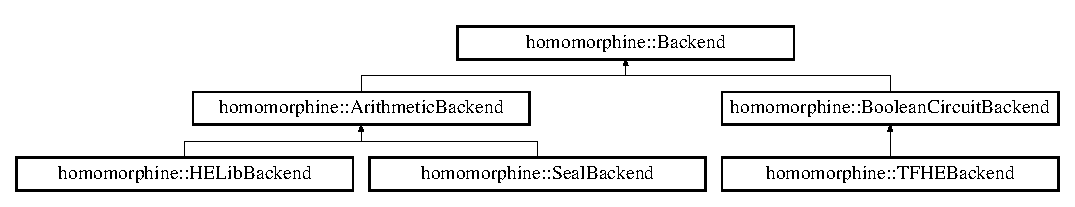
\includegraphics[height=2.333333cm]{classhomomorphine_1_1_backend}
\end{center}
\end{figure}
\subsection*{Public Member Functions}
\begin{DoxyCompactItemize}
\item 
map$<$ string, string $>$ \hyperlink{classhomomorphine_1_1_backend_a107e05b3bd55271356a57fbc0c1df091}{get\+Params} ()
\item 
void \hyperlink{classhomomorphine_1_1_backend_aed04b9aa4eb2c08801e099b16b4da4b0}{set\+Params} (map$<$ string, string $>$ \&params)
\item 
string \hyperlink{classhomomorphine_1_1_backend_a34191d0dbdd9e300a88242156f90eb9b}{get\+Param} (string key)
\item 
void \hyperlink{classhomomorphine_1_1_backend_aacb924f4de6d50347d550da85aec15a2}{set\+Param} (string \&key, string \&value)
\end{DoxyCompactItemize}


\subsection{Detailed Description}
/brief \hyperlink{classhomomorphine_1_1_backend}{Backend} interface

Provides an interface that each specific arithmetic backend has to provide 

\subsection{Member Function Documentation}
\mbox{\Hypertarget{classhomomorphine_1_1_backend_a34191d0dbdd9e300a88242156f90eb9b}\label{classhomomorphine_1_1_backend_a34191d0dbdd9e300a88242156f90eb9b}} 
\index{homomorphine\+::\+Backend@{homomorphine\+::\+Backend}!get\+Param@{get\+Param}}
\index{get\+Param@{get\+Param}!homomorphine\+::\+Backend@{homomorphine\+::\+Backend}}
\subsubsection{\texorpdfstring{get\+Param()}{getParam()}}
{\footnotesize\ttfamily string homomorphine\+::\+Backend\+::get\+Param (\begin{DoxyParamCaption}\item[{string}]{key }\end{DoxyParamCaption})}

Returns the specific parameter


\begin{DoxyParams}{Parameters}
{\em key} & parameter name \\
\hline
\end{DoxyParams}
\begin{DoxyReturn}{Returns}
parameter value 
\end{DoxyReturn}
\mbox{\Hypertarget{classhomomorphine_1_1_backend_a107e05b3bd55271356a57fbc0c1df091}\label{classhomomorphine_1_1_backend_a107e05b3bd55271356a57fbc0c1df091}} 
\index{homomorphine\+::\+Backend@{homomorphine\+::\+Backend}!get\+Params@{get\+Params}}
\index{get\+Params@{get\+Params}!homomorphine\+::\+Backend@{homomorphine\+::\+Backend}}
\subsubsection{\texorpdfstring{get\+Params()}{getParams()}}
{\footnotesize\ttfamily map$<$ string, string $>$ homomorphine\+::\+Backend\+::get\+Params (\begin{DoxyParamCaption}{ }\end{DoxyParamCaption})}

Returns the map of the params that have been set

\begin{DoxyReturn}{Returns}
map of params 
\end{DoxyReturn}
\mbox{\Hypertarget{classhomomorphine_1_1_backend_aacb924f4de6d50347d550da85aec15a2}\label{classhomomorphine_1_1_backend_aacb924f4de6d50347d550da85aec15a2}} 
\index{homomorphine\+::\+Backend@{homomorphine\+::\+Backend}!set\+Param@{set\+Param}}
\index{set\+Param@{set\+Param}!homomorphine\+::\+Backend@{homomorphine\+::\+Backend}}
\subsubsection{\texorpdfstring{set\+Param()}{setParam()}}
{\footnotesize\ttfamily void homomorphine\+::\+Backend\+::set\+Param (\begin{DoxyParamCaption}\item[{string \&}]{key,  }\item[{string \&}]{value }\end{DoxyParamCaption})}

Sets the specific parameter


\begin{DoxyParams}{Parameters}
{\em key} & parameter name \\
\hline
{\em value} & parameter value \\
\hline
\end{DoxyParams}
\mbox{\Hypertarget{classhomomorphine_1_1_backend_aed04b9aa4eb2c08801e099b16b4da4b0}\label{classhomomorphine_1_1_backend_aed04b9aa4eb2c08801e099b16b4da4b0}} 
\index{homomorphine\+::\+Backend@{homomorphine\+::\+Backend}!set\+Params@{set\+Params}}
\index{set\+Params@{set\+Params}!homomorphine\+::\+Backend@{homomorphine\+::\+Backend}}
\subsubsection{\texorpdfstring{set\+Params()}{setParams()}}
{\footnotesize\ttfamily void homomorphine\+::\+Backend\+::set\+Params (\begin{DoxyParamCaption}\item[{map$<$ string, string $>$ \&}]{params }\end{DoxyParamCaption})}

Sets the map of the params


\begin{DoxyParams}{Parameters}
{\em params} & map of params \\
\hline
\end{DoxyParams}


The documentation for this class was generated from the following files\+:\begin{DoxyCompactItemize}
\item 
src/backend.\+hpp\item 
src/backend.\+cpp\end{DoxyCompactItemize}

\hypertarget{classhomomorphine_1_1_backend_exception}{}\section{homomorphine\+::Backend\+Exception Class Reference}
\label{classhomomorphine_1_1_backend_exception}\index{homomorphine::BackendException@{homomorphine::BackendException}}


{\ttfamily \#include $<$backend.\+hpp$>$}

Inheritance diagram for homomorphine\+::Backend\+Exception\+:\begin{figure}[H]
\begin{center}
\leavevmode
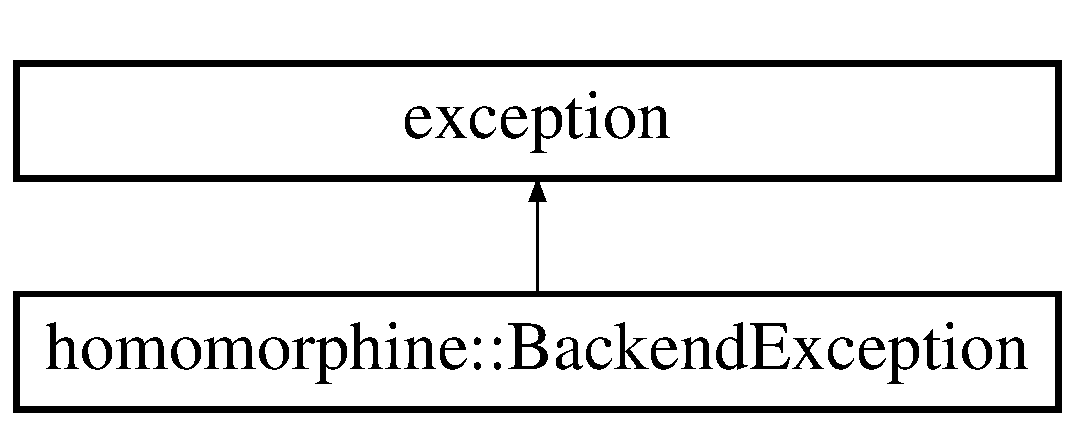
\includegraphics[height=2.000000cm]{classhomomorphine_1_1_backend_exception}
\end{center}
\end{figure}
\subsection*{Public Member Functions}
\begin{DoxyCompactItemize}
\item 
\mbox{\Hypertarget{classhomomorphine_1_1_backend_exception_add89cd603a906324b3d9f899c71bab50}\label{classhomomorphine_1_1_backend_exception_add89cd603a906324b3d9f899c71bab50}} 
{\bfseries Backend\+Exception} (const char $\ast$msg)
\item 
\mbox{\Hypertarget{classhomomorphine_1_1_backend_exception_a5b6595c44ccf8e2196c7989f695d71a4}\label{classhomomorphine_1_1_backend_exception_a5b6595c44ccf8e2196c7989f695d71a4}} 
const char $\ast$ {\bfseries get\+Message} ()
\end{DoxyCompactItemize}


\subsection{Detailed Description}
/brief \mbox{\hyperlink{classhomomorphine_1_1_backend}{Backend}} exception.

Thrown in case of a fatal error of specific backend implementation. 

The documentation for this class was generated from the following files\+:\begin{DoxyCompactItemize}
\item 
src/backend.\+hpp\item 
src/backend.\+cpp\end{DoxyCompactItemize}

\hypertarget{classhomomorphine_1_1_backend_operation_not_supported}{}\section{homomorphine\+::Backend\+Operation\+Not\+Supported Class Reference}
\label{classhomomorphine_1_1_backend_operation_not_supported}\index{homomorphine::BackendOperationNotSupported@{homomorphine::BackendOperationNotSupported}}


{\ttfamily \#include $<$arithmetic\+\_\+backend.\+hpp$>$}

Inheritance diagram for homomorphine\+::Backend\+Operation\+Not\+Supported\+:\begin{figure}[H]
\begin{center}
\leavevmode
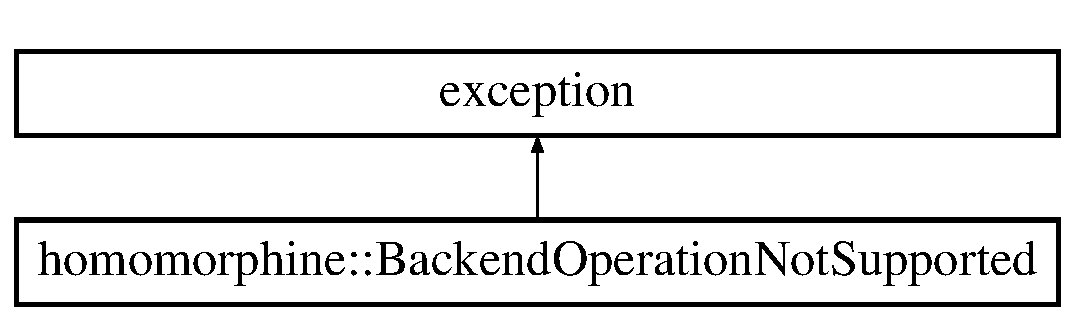
\includegraphics[height=2.000000cm]{classhomomorphine_1_1_backend_operation_not_supported}
\end{center}
\end{figure}
\subsection*{Public Member Functions}
\begin{DoxyCompactItemize}
\item 
\mbox{\Hypertarget{classhomomorphine_1_1_backend_operation_not_supported_a8db72ebb31be4189807aa36fec1ee927}\label{classhomomorphine_1_1_backend_operation_not_supported_a8db72ebb31be4189807aa36fec1ee927}} 
{\bfseries Backend\+Operation\+Not\+Supported} (const char $\ast$msg)
\item 
\mbox{\Hypertarget{classhomomorphine_1_1_backend_operation_not_supported_a909fc0802c577f246d5400baba44da45}\label{classhomomorphine_1_1_backend_operation_not_supported_a909fc0802c577f246d5400baba44da45}} 
const char $\ast$ {\bfseries get\+Message} ()
\end{DoxyCompactItemize}


\subsection{Detailed Description}
/brief Backend operation exception.

Thrown in case specific Backend can\textquotesingle{}t provide, or resolve a specific operation (i.\+e. not all arithmetic operations are provided by each backend). 

The documentation for this class was generated from the following files\+:\begin{DoxyCompactItemize}
\item 
src/arithmetic\+\_\+backend.\+hpp\item 
src/arithmetic\+\_\+backend.\+cpp\end{DoxyCompactItemize}

\input{classhomomorphine_1_1_boolean_circuit_backend}
\input{classhomomorphine_1_1_boolean_circuit_backend_factory}
\input{classhomomorphine_1_1_boolean_circuit_backend_factory_exception}
\hypertarget{classhomomorphine_1_1_config}{}\section{homomorphine\+::Config Class Reference}
\label{classhomomorphine_1_1_config}\index{homomorphine::Config@{homomorphine::Config}}


{\ttfamily \#include $<$config.\+hpp$>$}

\subsection*{Public Member Functions}
\begin{DoxyCompactItemize}
\item 
void \mbox{\hyperlink{classhomomorphine_1_1_config_ae3df94f615e3bc738525626875715a92}{init}} (string \&file)
\item 
map$<$ string, \mbox{\hyperlink{classhomomorphine_1_1_interface}{Interface}} $>$ \mbox{\hyperlink{classhomomorphine_1_1_config_a9286b3174aa24eddfe209fbe35fce303}{get\+Interfaces}} ()
\item 
int \mbox{\hyperlink{classhomomorphine_1_1_config_a48768be288a3e95be68488c02ce19601}{interfaces\+Size}} ()
\end{DoxyCompactItemize}
\subsection*{Friends}
\begin{DoxyCompactItemize}
\item 
\mbox{\Hypertarget{classhomomorphine_1_1_config_ad47f2707e919427dd6f15ccf25608b32}\label{classhomomorphine_1_1_config_ad47f2707e919427dd6f15ccf25608b32}} 
ostream \& {\bfseries operator$<$$<$} (ostream \&, const \mbox{\hyperlink{classhomomorphine_1_1_config}{Config}} \&)
\end{DoxyCompactItemize}


\subsection{Detailed Description}
/brief Configuration for Homomorphine service.

This class provides a configuration for Homomorphine service wrapper. 

\subsection{Member Function Documentation}
\mbox{\Hypertarget{classhomomorphine_1_1_config_a9286b3174aa24eddfe209fbe35fce303}\label{classhomomorphine_1_1_config_a9286b3174aa24eddfe209fbe35fce303}} 
\index{homomorphine::Config@{homomorphine::Config}!getInterfaces@{getInterfaces}}
\index{getInterfaces@{getInterfaces}!homomorphine::Config@{homomorphine::Config}}
\subsubsection{\texorpdfstring{getInterfaces()}{getInterfaces()}}
{\footnotesize\ttfamily map$<$ string, \mbox{\hyperlink{classhomomorphine_1_1_interface}{Interface}} $>$ homomorphine\+::\+Config\+::get\+Interfaces (\begin{DoxyParamCaption}{ }\end{DoxyParamCaption})}

Returns the configured interfaces.

\begin{DoxyReturn}{Returns}
map of interfaces 
\end{DoxyReturn}
\mbox{\Hypertarget{classhomomorphine_1_1_config_ae3df94f615e3bc738525626875715a92}\label{classhomomorphine_1_1_config_ae3df94f615e3bc738525626875715a92}} 
\index{homomorphine::Config@{homomorphine::Config}!init@{init}}
\index{init@{init}!homomorphine::Config@{homomorphine::Config}}
\subsubsection{\texorpdfstring{init()}{init()}}
{\footnotesize\ttfamily void homomorphine\+::\+Config\+::init (\begin{DoxyParamCaption}\item[{string \&}]{file }\end{DoxyParamCaption})}

Initialize configuration from J\+S\+ON file.


\begin{DoxyParams}{Parameters}
{\em file} & path to J\+S\+ON file \\
\hline
\end{DoxyParams}
\mbox{\Hypertarget{classhomomorphine_1_1_config_a48768be288a3e95be68488c02ce19601}\label{classhomomorphine_1_1_config_a48768be288a3e95be68488c02ce19601}} 
\index{homomorphine::Config@{homomorphine::Config}!interfacesSize@{interfacesSize}}
\index{interfacesSize@{interfacesSize}!homomorphine::Config@{homomorphine::Config}}
\subsubsection{\texorpdfstring{interfacesSize()}{interfacesSize()}}
{\footnotesize\ttfamily int homomorphine\+::\+Config\+::interfaces\+Size (\begin{DoxyParamCaption}{ }\end{DoxyParamCaption})}

Returns the number of interfaces.

\begin{DoxyReturn}{Returns}
number of interfaces 
\end{DoxyReturn}


The documentation for this class was generated from the following files\+:\begin{DoxyCompactItemize}
\item 
src/config.\+hpp\item 
src/config.\+cpp\end{DoxyCompactItemize}

\hypertarget{classhomomorphine_1_1_constants}{}\section{homomorphine\+::Constants Class Reference}
\label{classhomomorphine_1_1_constants}\index{homomorphine::Constants@{homomorphine::Constants}}


{\ttfamily \#include $<$constants.\+hpp$>$}

\subsection*{Static Public Attributes}
\begin{DoxyCompactItemize}
\item 
\mbox{\Hypertarget{classhomomorphine_1_1_constants_a354ff8671160245be639213c335a47dd}\label{classhomomorphine_1_1_constants_a354ff8671160245be639213c335a47dd}} 
static const int {\bfseries S\+E\+A\+L\+\_\+\+P\+O\+L\+Y\+\_\+\+M\+O\+D\+U\+L\+U\+S\+\_\+\+D\+E\+G\+R\+E\+E\+\_\+\+B\+FV} = 4096
\item 
\mbox{\Hypertarget{classhomomorphine_1_1_constants_acc9b94c27229e11b88f013eb4c09f526}\label{classhomomorphine_1_1_constants_acc9b94c27229e11b88f013eb4c09f526}} 
static const int {\bfseries S\+E\+A\+L\+\_\+\+P\+O\+L\+Y\+\_\+\+M\+O\+D\+U\+L\+U\+S\+\_\+\+D\+E\+G\+R\+E\+E\+\_\+\+C\+K\+KS} = 8192
\item 
\mbox{\Hypertarget{classhomomorphine_1_1_constants_ad87143078aecc13a757523a87ca5f6c1}\label{classhomomorphine_1_1_constants_ad87143078aecc13a757523a87ca5f6c1}} 
static const uint64\+\_\+t {\bfseries S\+E\+A\+L\+\_\+\+C\+O\+E\+F\+F\+\_\+\+M\+O\+D\+U\+L\+US} = 4096
\item 
\mbox{\Hypertarget{classhomomorphine_1_1_constants_a4fea8db185713db5b7c0a9b455adb06e}\label{classhomomorphine_1_1_constants_a4fea8db185713db5b7c0a9b455adb06e}} 
static const int {\bfseries S\+E\+A\+L\+\_\+\+P\+L\+A\+I\+N\+\_\+\+M\+O\+D\+U\+L\+US} = 40961
\item 
\mbox{\Hypertarget{classhomomorphine_1_1_constants_ab10b8c769059fcf9f04f16963c384677}\label{classhomomorphine_1_1_constants_ab10b8c769059fcf9f04f16963c384677}} 
static constexpr double {\bfseries S\+E\+A\+L\+\_\+\+C\+K\+K\+S\+\_\+\+S\+C\+A\+LE} = 1152921504606846976.\+0
\item 
\mbox{\Hypertarget{classhomomorphine_1_1_constants_a3eb0cdf60add8c31fdb68c1df36fd27c}\label{classhomomorphine_1_1_constants_a3eb0cdf60add8c31fdb68c1df36fd27c}} 
static const int {\bfseries S\+E\+A\+L\+\_\+\+S\+E\+C\+U\+R\+I\+T\+Y\+\_\+\+L\+E\+V\+EL} = 128
\item 
\mbox{\Hypertarget{classhomomorphine_1_1_constants_a25426ff47774d7ff0b88a0f7af1cfbb5}\label{classhomomorphine_1_1_constants_a25426ff47774d7ff0b88a0f7af1cfbb5}} 
static const unsigned long {\bfseries H\+E\+L\+I\+B\+\_\+\+P\+L\+A\+I\+N\+T\+E\+X\+T\+\_\+\+P\+R\+I\+M\+E\+\_\+\+M\+O\+D\+U\+L\+US} = 997
\item 
\mbox{\Hypertarget{classhomomorphine_1_1_constants_a1392b13d6e1546225b95928311e53e85}\label{classhomomorphine_1_1_constants_a1392b13d6e1546225b95928311e53e85}} 
static const unsigned long {\bfseries H\+E\+L\+I\+B\+\_\+\+H\+E\+N\+S\+E\+L\+\_\+\+L\+I\+F\+T\+I\+NG} = 1
\item 
\mbox{\Hypertarget{classhomomorphine_1_1_constants_a0dff16e6343989a60f4833605e45525f}\label{classhomomorphine_1_1_constants_a0dff16e6343989a60f4833605e45525f}} 
static const unsigned long {\bfseries H\+E\+L\+I\+B\+\_\+\+M\+O\+D\+U\+L\+U\+S\+\_\+\+C\+H\+A\+I\+N\+\_\+\+B\+I\+TS} = 32
\item 
\mbox{\Hypertarget{classhomomorphine_1_1_constants_af08d97d4333bf772d742dddb6cac3af7}\label{classhomomorphine_1_1_constants_af08d97d4333bf772d742dddb6cac3af7}} 
static const unsigned long {\bfseries H\+E\+L\+I\+B\+\_\+\+N\+U\+M\+B\+E\+R\+\_\+\+O\+F\+\_\+\+C\+O\+L\+U\+M\+NS} = 2
\item 
\mbox{\Hypertarget{classhomomorphine_1_1_constants_a86e3b8595c5ea2ed0be83f454dcc22d9}\label{classhomomorphine_1_1_constants_a86e3b8595c5ea2ed0be83f454dcc22d9}} 
static const unsigned long {\bfseries H\+E\+L\+I\+B\+\_\+\+H\+A\+M\+M\+I\+N\+G\+\_\+\+W\+E\+I\+G\+HT} = 64
\item 
\mbox{\Hypertarget{classhomomorphine_1_1_constants_a043276f012d91267f62249aee29dfc04}\label{classhomomorphine_1_1_constants_a043276f012d91267f62249aee29dfc04}} 
static const unsigned long {\bfseries H\+E\+L\+I\+B\+\_\+\+S\+E\+C\+U\+R\+I\+T\+Y\+\_\+\+L\+E\+V\+EL} = 128
\item 
\mbox{\Hypertarget{classhomomorphine_1_1_constants_aac8aee7a978989ff544b02f8534fff24}\label{classhomomorphine_1_1_constants_aac8aee7a978989ff544b02f8534fff24}} 
static const unsigned long {\bfseries H\+E\+L\+I\+B\+\_\+\+D\+E\+G\+R\+E\+E\+\_\+\+O\+F\+\_\+\+F\+I\+E\+L\+D\+\_\+\+E\+X\+T\+E\+N\+S\+I\+ON} = 0
\item 
\mbox{\Hypertarget{classhomomorphine_1_1_constants_a94ae2d93d643d610ef822f8a06dde37f}\label{classhomomorphine_1_1_constants_a94ae2d93d643d610ef822f8a06dde37f}} 
static const unsigned long {\bfseries H\+E\+L\+I\+B\+\_\+\+M\+I\+N\+I\+M\+U\+M\+\_\+\+N\+U\+M\+B\+E\+R\+\_\+\+O\+F\+\_\+\+S\+L\+O\+TS} = 0
\item 
\mbox{\Hypertarget{classhomomorphine_1_1_constants_aa8ea7bb198826c9458fe8b975c1dcd64}\label{classhomomorphine_1_1_constants_aa8ea7bb198826c9458fe8b975c1dcd64}} 
static const int {\bfseries T\+F\+H\+E\+\_\+\+R\+A\+N\+D\+O\+M\+\_\+\+D\+E\+P\+TH} = 3
\item 
\mbox{\Hypertarget{classhomomorphine_1_1_constants_a8581d42bf2a8ffa81c2760f7fdd3c8a3}\label{classhomomorphine_1_1_constants_a8581d42bf2a8ffa81c2760f7fdd3c8a3}} 
static const int {\bfseries T\+F\+H\+E\+\_\+\+M\+I\+N\+I\+M\+U\+M\+\_\+\+L\+A\+M\+B\+DA} = 110
\item 
\mbox{\Hypertarget{classhomomorphine_1_1_constants_a7c01eca379ffe908e8b4b2bc22e2d24a}\label{classhomomorphine_1_1_constants_a7c01eca379ffe908e8b4b2bc22e2d24a}} 
static const int {\bfseries T\+F\+H\+E\+\_\+\+B\+I\+T\+S\+\_\+\+E\+N\+C\+R\+Y\+PT} = 16
\end{DoxyCompactItemize}


\subsection{Detailed Description}
/brief Default value container

Provides default values for certain parameters used by specific homomorphic encryption backends 

The documentation for this class was generated from the following file\+:\begin{DoxyCompactItemize}
\item 
src/constants.\+hpp\end{DoxyCompactItemize}

\hypertarget{classhomomorphine_1_1_h_e_lib_backend}{}\section{homomorphine\+::H\+E\+Lib\+Backend Class Reference}
\label{classhomomorphine_1_1_h_e_lib_backend}\index{homomorphine::HELibBackend@{homomorphine::HELibBackend}}


{\ttfamily \#include $<$helib\+\_\+backend.\+hpp$>$}

Inheritance diagram for homomorphine\+::H\+E\+Lib\+Backend\+:\begin{figure}[H]
\begin{center}
\leavevmode
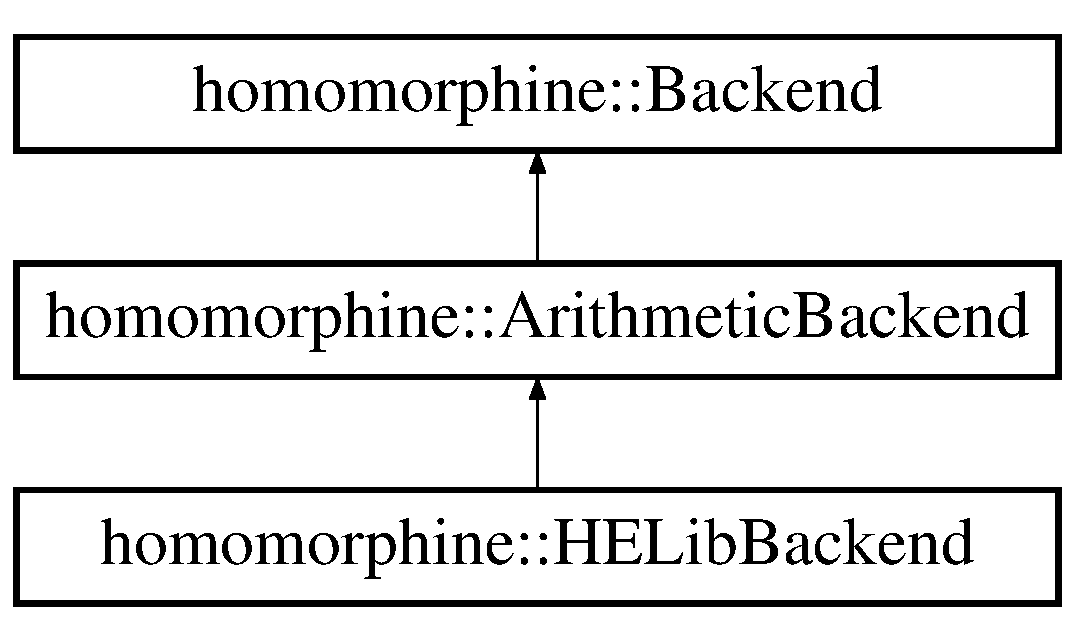
\includegraphics[height=3.000000cm]{classhomomorphine_1_1_h_e_lib_backend}
\end{center}
\end{figure}
\subsection*{Public Member Functions}
\begin{DoxyCompactItemize}
\item 
\mbox{\hyperlink{classhomomorphine_1_1_h_e_lib_backend_a1ef98efe05281fefbe6d044dc474017a}{$\sim$\+H\+E\+Lib\+Backend}} ()
\item 
void \mbox{\hyperlink{classhomomorphine_1_1_h_e_lib_backend_a39478377b0e299fd90f5c7bb6c8efe89}{set\+Algorithm}} (string algorithm)
\item 
void \mbox{\hyperlink{classhomomorphine_1_1_h_e_lib_backend_a6a7e7c8095f2287c41f7d93be91418ec}{init}} ()
\item 
void \mbox{\hyperlink{classhomomorphine_1_1_h_e_lib_backend_a2c6ed82eeb597b99ae6cdb2734412a0f}{generate\+Keys}} ()
\item 
string \mbox{\hyperlink{classhomomorphine_1_1_h_e_lib_backend_a8b096d4780f3b65f0fa0cb3ca6cb9ab8}{get\+Public\+Key}} ()
\item 
string \mbox{\hyperlink{classhomomorphine_1_1_h_e_lib_backend_a57af39a901a44fef6aad76503739fde4}{get\+Secret\+Key}} ()
\item 
pair$<$ string, string $>$ \mbox{\hyperlink{classhomomorphine_1_1_h_e_lib_backend_ab45838cc01a4e71425e2aa0279e12c0e}{get\+Keys}} ()
\item 
void \mbox{\hyperlink{classhomomorphine_1_1_h_e_lib_backend_af54dc3990d99aab69c97172d0e5b4e51}{set\+Public\+Key}} (string public\+\_\+key)
\item 
void \mbox{\hyperlink{classhomomorphine_1_1_h_e_lib_backend_a483a6695be2d733d48e2180ffb25d053}{set\+Secret\+Key}} (string secret\+\_\+key)
\item 
void \mbox{\hyperlink{classhomomorphine_1_1_h_e_lib_backend_a2980c8eaf3556057aac364a1e61ab8cd}{set\+Keys}} (string public\+\_\+key, string secret\+\_\+key)
\item 
string \mbox{\hyperlink{classhomomorphine_1_1_h_e_lib_backend_a9ba4311289e3b8c47f389f4f44de7d5d}{get\+Cipher}} ()
\item 
void \mbox{\hyperlink{classhomomorphine_1_1_h_e_lib_backend_a5baa6ad05fbb23d27c4ec4bb018a8c64}{set\+Cipher}} (string cipher)
\item 
string \mbox{\hyperlink{classhomomorphine_1_1_h_e_lib_backend_af030a10bdd905f7cccf72c8eabfefdd7}{encrypt}} (vector$<$ long $>$ values)
\item 
string \mbox{\hyperlink{classhomomorphine_1_1_h_e_lib_backend_a6a958824a123eab41b2099dbc001dc13}{encrypt}} (long value)
\item 
vector$<$ long $>$ \mbox{\hyperlink{classhomomorphine_1_1_h_e_lib_backend_a650d87bee6056a404f8ab81ec0f84980}{decrypt\+Values}} ()
\item 
long \mbox{\hyperlink{classhomomorphine_1_1_h_e_lib_backend_a2cd3ebc5a3332100e6cb24480262c395}{decrypt}} ()
\item 
void \mbox{\hyperlink{classhomomorphine_1_1_h_e_lib_backend_a1e3c4745d7efdaac1f75c5a7fbfc3707}{add}} (vector$<$ long $>$ values)
\item 
void \mbox{\hyperlink{classhomomorphine_1_1_h_e_lib_backend_a6cc00dcfc209206e67c7237934cb8d82}{add}} (long value)
\item 
void \mbox{\hyperlink{classhomomorphine_1_1_h_e_lib_backend_acb1ed456fa91fc1dfe878abb068f3f34}{negate}} ()
\item 
void \mbox{\hyperlink{classhomomorphine_1_1_h_e_lib_backend_a05b508bcc4a165d045ebc09f190c5a95}{multiply}} (vector$<$ long $>$ values)
\item 
void \mbox{\hyperlink{classhomomorphine_1_1_h_e_lib_backend_a49d4e073eecc4759f12f60188a533835}{multiply}} (long value)
\end{DoxyCompactItemize}
\subsection*{Additional Inherited Members}


\subsection{Detailed Description}
/brief H\+E\+Lib backend

This class is an implementation of the S\+E\+AL backend. 

\subsection{Constructor \& Destructor Documentation}
\mbox{\Hypertarget{classhomomorphine_1_1_h_e_lib_backend_a1ef98efe05281fefbe6d044dc474017a}\label{classhomomorphine_1_1_h_e_lib_backend_a1ef98efe05281fefbe6d044dc474017a}} 
\index{homomorphine::HELibBackend@{homomorphine::HELibBackend}!````~HELibBackend@{$\sim$HELibBackend}}
\index{````~HELibBackend@{$\sim$HELibBackend}!homomorphine::HELibBackend@{homomorphine::HELibBackend}}
\subsubsection{\texorpdfstring{$\sim$HELibBackend()}{~HELibBackend()}}
{\footnotesize\ttfamily homomorphine\+::\+H\+E\+Lib\+Backend\+::$\sim$\+H\+E\+Lib\+Backend (\begin{DoxyParamCaption}{ }\end{DoxyParamCaption})}

H\+E\+Lib backend cleanup 

\subsection{Member Function Documentation}
\mbox{\Hypertarget{classhomomorphine_1_1_h_e_lib_backend_a1e3c4745d7efdaac1f75c5a7fbfc3707}\label{classhomomorphine_1_1_h_e_lib_backend_a1e3c4745d7efdaac1f75c5a7fbfc3707}} 
\index{homomorphine::HELibBackend@{homomorphine::HELibBackend}!add@{add}}
\index{add@{add}!homomorphine::HELibBackend@{homomorphine::HELibBackend}}
\subsubsection{\texorpdfstring{add()}{add()}\hspace{0.1cm}{\footnotesize\ttfamily [1/2]}}
{\footnotesize\ttfamily void homomorphine\+::\+H\+E\+Lib\+Backend\+::add (\begin{DoxyParamCaption}\item[{vector$<$ long $>$}]{values }\end{DoxyParamCaption})\hspace{0.3cm}{\ttfamily [virtual]}}

Adds the vector of values to encrypted vector of values


\begin{DoxyParams}{Parameters}
{\em values} & vector of values \\
\hline
\end{DoxyParams}


Implements \mbox{\hyperlink{classhomomorphine_1_1_arithmetic_backend_abf4053e05f07e566e9563a75f516daf6}{homomorphine\+::\+Arithmetic\+Backend}}.

\mbox{\Hypertarget{classhomomorphine_1_1_h_e_lib_backend_a6cc00dcfc209206e67c7237934cb8d82}\label{classhomomorphine_1_1_h_e_lib_backend_a6cc00dcfc209206e67c7237934cb8d82}} 
\index{homomorphine::HELibBackend@{homomorphine::HELibBackend}!add@{add}}
\index{add@{add}!homomorphine::HELibBackend@{homomorphine::HELibBackend}}
\subsubsection{\texorpdfstring{add()}{add()}\hspace{0.1cm}{\footnotesize\ttfamily [2/2]}}
{\footnotesize\ttfamily void homomorphine\+::\+H\+E\+Lib\+Backend\+::add (\begin{DoxyParamCaption}\item[{long}]{value }\end{DoxyParamCaption})\hspace{0.3cm}{\ttfamily [virtual]}}

Adds the value to encrypted value


\begin{DoxyParams}{Parameters}
{\em value} & value \\
\hline
\end{DoxyParams}


Implements \mbox{\hyperlink{classhomomorphine_1_1_arithmetic_backend_aa1c88ebc894527a72a9fdbd35ca14204}{homomorphine\+::\+Arithmetic\+Backend}}.

\mbox{\Hypertarget{classhomomorphine_1_1_h_e_lib_backend_a2cd3ebc5a3332100e6cb24480262c395}\label{classhomomorphine_1_1_h_e_lib_backend_a2cd3ebc5a3332100e6cb24480262c395}} 
\index{homomorphine::HELibBackend@{homomorphine::HELibBackend}!decrypt@{decrypt}}
\index{decrypt@{decrypt}!homomorphine::HELibBackend@{homomorphine::HELibBackend}}
\subsubsection{\texorpdfstring{decrypt()}{decrypt()}}
{\footnotesize\ttfamily long homomorphine\+::\+H\+E\+Lib\+Backend\+::decrypt (\begin{DoxyParamCaption}{ }\end{DoxyParamCaption})\hspace{0.3cm}{\ttfamily [virtual]}}

Decrypts the single value using the secret key

\begin{DoxyReturn}{Returns}
decrypted value 
\end{DoxyReturn}


Implements \mbox{\hyperlink{classhomomorphine_1_1_arithmetic_backend_af4aad032c46ce51e608092ac206882bd}{homomorphine\+::\+Arithmetic\+Backend}}.

\mbox{\Hypertarget{classhomomorphine_1_1_h_e_lib_backend_a650d87bee6056a404f8ab81ec0f84980}\label{classhomomorphine_1_1_h_e_lib_backend_a650d87bee6056a404f8ab81ec0f84980}} 
\index{homomorphine::HELibBackend@{homomorphine::HELibBackend}!decryptValues@{decryptValues}}
\index{decryptValues@{decryptValues}!homomorphine::HELibBackend@{homomorphine::HELibBackend}}
\subsubsection{\texorpdfstring{decryptValues()}{decryptValues()}}
{\footnotesize\ttfamily vector$<$ long $>$ homomorphine\+::\+H\+E\+Lib\+Backend\+::decrypt\+Values (\begin{DoxyParamCaption}{ }\end{DoxyParamCaption})\hspace{0.3cm}{\ttfamily [virtual]}}

Decrypts the vector of values using the secret key

\begin{DoxyReturn}{Returns}
vector of decrypted values 
\end{DoxyReturn}


Implements \mbox{\hyperlink{classhomomorphine_1_1_arithmetic_backend_a2fb1ce64e74c4930b7d364ce3b9cc8fe}{homomorphine\+::\+Arithmetic\+Backend}}.

\mbox{\Hypertarget{classhomomorphine_1_1_h_e_lib_backend_af030a10bdd905f7cccf72c8eabfefdd7}\label{classhomomorphine_1_1_h_e_lib_backend_af030a10bdd905f7cccf72c8eabfefdd7}} 
\index{homomorphine::HELibBackend@{homomorphine::HELibBackend}!encrypt@{encrypt}}
\index{encrypt@{encrypt}!homomorphine::HELibBackend@{homomorphine::HELibBackend}}
\subsubsection{\texorpdfstring{encrypt()}{encrypt()}\hspace{0.1cm}{\footnotesize\ttfamily [1/2]}}
{\footnotesize\ttfamily string homomorphine\+::\+H\+E\+Lib\+Backend\+::encrypt (\begin{DoxyParamCaption}\item[{vector$<$ long $>$}]{values }\end{DoxyParamCaption})\hspace{0.3cm}{\ttfamily [virtual]}}

Encrypts the vector of values using the public key


\begin{DoxyParams}{Parameters}
{\em values} & vector of values \\
\hline
\end{DoxyParams}
\begin{DoxyReturn}{Returns}
U\+U\+Encoded cipher 
\end{DoxyReturn}


Implements \mbox{\hyperlink{classhomomorphine_1_1_arithmetic_backend_ae97a4987b6024961d8b70a4a0ad2d653}{homomorphine\+::\+Arithmetic\+Backend}}.

\mbox{\Hypertarget{classhomomorphine_1_1_h_e_lib_backend_a6a958824a123eab41b2099dbc001dc13}\label{classhomomorphine_1_1_h_e_lib_backend_a6a958824a123eab41b2099dbc001dc13}} 
\index{homomorphine::HELibBackend@{homomorphine::HELibBackend}!encrypt@{encrypt}}
\index{encrypt@{encrypt}!homomorphine::HELibBackend@{homomorphine::HELibBackend}}
\subsubsection{\texorpdfstring{encrypt()}{encrypt()}\hspace{0.1cm}{\footnotesize\ttfamily [2/2]}}
{\footnotesize\ttfamily string homomorphine\+::\+H\+E\+Lib\+Backend\+::encrypt (\begin{DoxyParamCaption}\item[{long}]{value }\end{DoxyParamCaption})\hspace{0.3cm}{\ttfamily [virtual]}}

Encrypts the single value using the public key


\begin{DoxyParams}{Parameters}
{\em value} & value \\
\hline
\end{DoxyParams}
\begin{DoxyReturn}{Returns}
U\+U\+Encoded cipher 
\end{DoxyReturn}


Implements \mbox{\hyperlink{classhomomorphine_1_1_arithmetic_backend_ad6aedf61ae1a6257e81bd415ec08ac17}{homomorphine\+::\+Arithmetic\+Backend}}.

\mbox{\Hypertarget{classhomomorphine_1_1_h_e_lib_backend_a2c6ed82eeb597b99ae6cdb2734412a0f}\label{classhomomorphine_1_1_h_e_lib_backend_a2c6ed82eeb597b99ae6cdb2734412a0f}} 
\index{homomorphine::HELibBackend@{homomorphine::HELibBackend}!generateKeys@{generateKeys}}
\index{generateKeys@{generateKeys}!homomorphine::HELibBackend@{homomorphine::HELibBackend}}
\subsubsection{\texorpdfstring{generateKeys()}{generateKeys()}}
{\footnotesize\ttfamily void homomorphine\+::\+H\+E\+Lib\+Backend\+::generate\+Keys (\begin{DoxyParamCaption}{ }\end{DoxyParamCaption})\hspace{0.3cm}{\ttfamily [virtual]}}

Generates the public/secret key pair 

Implements \mbox{\hyperlink{classhomomorphine_1_1_arithmetic_backend_a5faa0089b80be5629d4a0a7a02fe3568}{homomorphine\+::\+Arithmetic\+Backend}}.

\mbox{\Hypertarget{classhomomorphine_1_1_h_e_lib_backend_a9ba4311289e3b8c47f389f4f44de7d5d}\label{classhomomorphine_1_1_h_e_lib_backend_a9ba4311289e3b8c47f389f4f44de7d5d}} 
\index{homomorphine::HELibBackend@{homomorphine::HELibBackend}!getCipher@{getCipher}}
\index{getCipher@{getCipher}!homomorphine::HELibBackend@{homomorphine::HELibBackend}}
\subsubsection{\texorpdfstring{getCipher()}{getCipher()}}
{\footnotesize\ttfamily string homomorphine\+::\+H\+E\+Lib\+Backend\+::get\+Cipher (\begin{DoxyParamCaption}{ }\end{DoxyParamCaption})\hspace{0.3cm}{\ttfamily [virtual]}}

Returns the U\+U\+Encoded cipher containing ecrypted value, or vector of values

\begin{DoxyReturn}{Returns}
U\+U\+Encoded cipher 
\end{DoxyReturn}


Implements \mbox{\hyperlink{classhomomorphine_1_1_arithmetic_backend_acf38918fb556703ccb12b63dc73b15ed}{homomorphine\+::\+Arithmetic\+Backend}}.

\mbox{\Hypertarget{classhomomorphine_1_1_h_e_lib_backend_ab45838cc01a4e71425e2aa0279e12c0e}\label{classhomomorphine_1_1_h_e_lib_backend_ab45838cc01a4e71425e2aa0279e12c0e}} 
\index{homomorphine::HELibBackend@{homomorphine::HELibBackend}!getKeys@{getKeys}}
\index{getKeys@{getKeys}!homomorphine::HELibBackend@{homomorphine::HELibBackend}}
\subsubsection{\texorpdfstring{getKeys()}{getKeys()}}
{\footnotesize\ttfamily pair$<$ string, string $>$ homomorphine\+::\+H\+E\+Lib\+Backend\+::get\+Keys (\begin{DoxyParamCaption}{ }\end{DoxyParamCaption})\hspace{0.3cm}{\ttfamily [virtual]}}

Returns the pair of U\+U\+Encoded public and secret keys

\begin{DoxyReturn}{Returns}
pair of public and secret keys 
\end{DoxyReturn}


Implements \mbox{\hyperlink{classhomomorphine_1_1_arithmetic_backend_a71bb86054685708001c636e3085d578c}{homomorphine\+::\+Arithmetic\+Backend}}.

\mbox{\Hypertarget{classhomomorphine_1_1_h_e_lib_backend_a8b096d4780f3b65f0fa0cb3ca6cb9ab8}\label{classhomomorphine_1_1_h_e_lib_backend_a8b096d4780f3b65f0fa0cb3ca6cb9ab8}} 
\index{homomorphine::HELibBackend@{homomorphine::HELibBackend}!getPublicKey@{getPublicKey}}
\index{getPublicKey@{getPublicKey}!homomorphine::HELibBackend@{homomorphine::HELibBackend}}
\subsubsection{\texorpdfstring{getPublicKey()}{getPublicKey()}}
{\footnotesize\ttfamily string homomorphine\+::\+H\+E\+Lib\+Backend\+::get\+Public\+Key (\begin{DoxyParamCaption}{ }\end{DoxyParamCaption})\hspace{0.3cm}{\ttfamily [virtual]}}

Returns the U\+U\+Encoded public key

\begin{DoxyReturn}{Returns}
public key 
\end{DoxyReturn}


Implements \mbox{\hyperlink{classhomomorphine_1_1_arithmetic_backend_a26f31fc0c76cf58636972f68142b9a06}{homomorphine\+::\+Arithmetic\+Backend}}.

\mbox{\Hypertarget{classhomomorphine_1_1_h_e_lib_backend_a57af39a901a44fef6aad76503739fde4}\label{classhomomorphine_1_1_h_e_lib_backend_a57af39a901a44fef6aad76503739fde4}} 
\index{homomorphine::HELibBackend@{homomorphine::HELibBackend}!getSecretKey@{getSecretKey}}
\index{getSecretKey@{getSecretKey}!homomorphine::HELibBackend@{homomorphine::HELibBackend}}
\subsubsection{\texorpdfstring{getSecretKey()}{getSecretKey()}}
{\footnotesize\ttfamily string homomorphine\+::\+H\+E\+Lib\+Backend\+::get\+Secret\+Key (\begin{DoxyParamCaption}{ }\end{DoxyParamCaption})\hspace{0.3cm}{\ttfamily [virtual]}}

Returns the U\+U\+Encoded secret key

\begin{DoxyReturn}{Returns}
secret key 
\end{DoxyReturn}


Implements \mbox{\hyperlink{classhomomorphine_1_1_arithmetic_backend_a679abf60fea83922f7972498c4500252}{homomorphine\+::\+Arithmetic\+Backend}}.

\mbox{\Hypertarget{classhomomorphine_1_1_h_e_lib_backend_a6a7e7c8095f2287c41f7d93be91418ec}\label{classhomomorphine_1_1_h_e_lib_backend_a6a7e7c8095f2287c41f7d93be91418ec}} 
\index{homomorphine::HELibBackend@{homomorphine::HELibBackend}!init@{init}}
\index{init@{init}!homomorphine::HELibBackend@{homomorphine::HELibBackend}}
\subsubsection{\texorpdfstring{init()}{init()}}
{\footnotesize\ttfamily void homomorphine\+::\+H\+E\+Lib\+Backend\+::init (\begin{DoxyParamCaption}{ }\end{DoxyParamCaption})\hspace{0.3cm}{\ttfamily [virtual]}}

Initializes the H\+E\+Lib backend 

Implements \mbox{\hyperlink{classhomomorphine_1_1_arithmetic_backend_a2654ee62a6cf2f16fd41c834a26b0006}{homomorphine\+::\+Arithmetic\+Backend}}.

\mbox{\Hypertarget{classhomomorphine_1_1_h_e_lib_backend_a05b508bcc4a165d045ebc09f190c5a95}\label{classhomomorphine_1_1_h_e_lib_backend_a05b508bcc4a165d045ebc09f190c5a95}} 
\index{homomorphine::HELibBackend@{homomorphine::HELibBackend}!multiply@{multiply}}
\index{multiply@{multiply}!homomorphine::HELibBackend@{homomorphine::HELibBackend}}
\subsubsection{\texorpdfstring{multiply()}{multiply()}\hspace{0.1cm}{\footnotesize\ttfamily [1/2]}}
{\footnotesize\ttfamily void homomorphine\+::\+H\+E\+Lib\+Backend\+::multiply (\begin{DoxyParamCaption}\item[{vector$<$ long $>$}]{values }\end{DoxyParamCaption})\hspace{0.3cm}{\ttfamily [virtual]}}

Multiplies the vector of values with the encrypted vector of values


\begin{DoxyParams}{Parameters}
{\em values} & vector of values \\
\hline
\end{DoxyParams}


Implements \mbox{\hyperlink{classhomomorphine_1_1_arithmetic_backend_a80f2424d26fcfad4803f6a0e5a9cdd2d}{homomorphine\+::\+Arithmetic\+Backend}}.

\mbox{\Hypertarget{classhomomorphine_1_1_h_e_lib_backend_a49d4e073eecc4759f12f60188a533835}\label{classhomomorphine_1_1_h_e_lib_backend_a49d4e073eecc4759f12f60188a533835}} 
\index{homomorphine::HELibBackend@{homomorphine::HELibBackend}!multiply@{multiply}}
\index{multiply@{multiply}!homomorphine::HELibBackend@{homomorphine::HELibBackend}}
\subsubsection{\texorpdfstring{multiply()}{multiply()}\hspace{0.1cm}{\footnotesize\ttfamily [2/2]}}
{\footnotesize\ttfamily void homomorphine\+::\+H\+E\+Lib\+Backend\+::multiply (\begin{DoxyParamCaption}\item[{long}]{value }\end{DoxyParamCaption})\hspace{0.3cm}{\ttfamily [virtual]}}

Multiplies the value with the encrypted value


\begin{DoxyParams}{Parameters}
{\em value} & value \\
\hline
\end{DoxyParams}


Implements \mbox{\hyperlink{classhomomorphine_1_1_arithmetic_backend_a22f4c598c5a3987ef6efe5925f4c5b81}{homomorphine\+::\+Arithmetic\+Backend}}.

\mbox{\Hypertarget{classhomomorphine_1_1_h_e_lib_backend_acb1ed456fa91fc1dfe878abb068f3f34}\label{classhomomorphine_1_1_h_e_lib_backend_acb1ed456fa91fc1dfe878abb068f3f34}} 
\index{homomorphine::HELibBackend@{homomorphine::HELibBackend}!negate@{negate}}
\index{negate@{negate}!homomorphine::HELibBackend@{homomorphine::HELibBackend}}
\subsubsection{\texorpdfstring{negate()}{negate()}}
{\footnotesize\ttfamily void homomorphine\+::\+H\+E\+Lib\+Backend\+::negate (\begin{DoxyParamCaption}{ }\end{DoxyParamCaption})\hspace{0.3cm}{\ttfamily [virtual]}}

Negates a single encrypted value, or a vector of encrypted values 

Implements \mbox{\hyperlink{classhomomorphine_1_1_arithmetic_backend_ad27913060534c42b5812a1e4cf21475f}{homomorphine\+::\+Arithmetic\+Backend}}.

\mbox{\Hypertarget{classhomomorphine_1_1_h_e_lib_backend_a39478377b0e299fd90f5c7bb6c8efe89}\label{classhomomorphine_1_1_h_e_lib_backend_a39478377b0e299fd90f5c7bb6c8efe89}} 
\index{homomorphine::HELibBackend@{homomorphine::HELibBackend}!setAlgorithm@{setAlgorithm}}
\index{setAlgorithm@{setAlgorithm}!homomorphine::HELibBackend@{homomorphine::HELibBackend}}
\subsubsection{\texorpdfstring{setAlgorithm()}{setAlgorithm()}}
{\footnotesize\ttfamily void homomorphine\+::\+H\+E\+Lib\+Backend\+::set\+Algorithm (\begin{DoxyParamCaption}\item[{string}]{algorithm }\end{DoxyParamCaption})\hspace{0.3cm}{\ttfamily [virtual]}}

Sets the specific H\+E\+Lib algorithm implementation that backend provides (currently, only default one)


\begin{DoxyParams}{Parameters}
{\em algorithm} & homomorphic encryption algorithm \\
\hline
\end{DoxyParams}


Implements \mbox{\hyperlink{classhomomorphine_1_1_arithmetic_backend_ac53135f4f66a2f7a33d3c6e6d465b86f}{homomorphine\+::\+Arithmetic\+Backend}}.

\mbox{\Hypertarget{classhomomorphine_1_1_h_e_lib_backend_a5baa6ad05fbb23d27c4ec4bb018a8c64}\label{classhomomorphine_1_1_h_e_lib_backend_a5baa6ad05fbb23d27c4ec4bb018a8c64}} 
\index{homomorphine::HELibBackend@{homomorphine::HELibBackend}!setCipher@{setCipher}}
\index{setCipher@{setCipher}!homomorphine::HELibBackend@{homomorphine::HELibBackend}}
\subsubsection{\texorpdfstring{setCipher()}{setCipher()}}
{\footnotesize\ttfamily void homomorphine\+::\+H\+E\+Lib\+Backend\+::set\+Cipher (\begin{DoxyParamCaption}\item[{string}]{cipher }\end{DoxyParamCaption})\hspace{0.3cm}{\ttfamily [virtual]}}

Sets the U\+U\+Encoded cipher containing ecrypted value, or vector of values


\begin{DoxyParams}{Parameters}
{\em cipher} & U\+U\+Encoded cipher \\
\hline
\end{DoxyParams}


Implements \mbox{\hyperlink{classhomomorphine_1_1_arithmetic_backend_af9b2d3b33a03d79facdf113c9560fc0b}{homomorphine\+::\+Arithmetic\+Backend}}.

\mbox{\Hypertarget{classhomomorphine_1_1_h_e_lib_backend_a2980c8eaf3556057aac364a1e61ab8cd}\label{classhomomorphine_1_1_h_e_lib_backend_a2980c8eaf3556057aac364a1e61ab8cd}} 
\index{homomorphine::HELibBackend@{homomorphine::HELibBackend}!setKeys@{setKeys}}
\index{setKeys@{setKeys}!homomorphine::HELibBackend@{homomorphine::HELibBackend}}
\subsubsection{\texorpdfstring{setKeys()}{setKeys()}}
{\footnotesize\ttfamily void homomorphine\+::\+H\+E\+Lib\+Backend\+::set\+Keys (\begin{DoxyParamCaption}\item[{string}]{public\+\_\+key,  }\item[{string}]{secret\+\_\+key }\end{DoxyParamCaption})\hspace{0.3cm}{\ttfamily [virtual]}}

Sets the both public and secret keys


\begin{DoxyParams}{Parameters}
{\em public\+\_\+key} & U\+U\+Encoded public key \\
\hline
{\em secret\+\_\+key} & U\+U\+Encoded secret key \\
\hline
\end{DoxyParams}


Implements \mbox{\hyperlink{classhomomorphine_1_1_arithmetic_backend_ac78f4b42dce3dce23edd81dba60b16c8}{homomorphine\+::\+Arithmetic\+Backend}}.

\mbox{\Hypertarget{classhomomorphine_1_1_h_e_lib_backend_af54dc3990d99aab69c97172d0e5b4e51}\label{classhomomorphine_1_1_h_e_lib_backend_af54dc3990d99aab69c97172d0e5b4e51}} 
\index{homomorphine::HELibBackend@{homomorphine::HELibBackend}!setPublicKey@{setPublicKey}}
\index{setPublicKey@{setPublicKey}!homomorphine::HELibBackend@{homomorphine::HELibBackend}}
\subsubsection{\texorpdfstring{setPublicKey()}{setPublicKey()}}
{\footnotesize\ttfamily void homomorphine\+::\+H\+E\+Lib\+Backend\+::set\+Public\+Key (\begin{DoxyParamCaption}\item[{string}]{public\+\_\+key }\end{DoxyParamCaption})\hspace{0.3cm}{\ttfamily [virtual]}}

Sets the public key


\begin{DoxyParams}{Parameters}
{\em public\+\_\+key} & U\+U\+Encoded public key \\
\hline
\end{DoxyParams}


Implements \mbox{\hyperlink{classhomomorphine_1_1_arithmetic_backend_af2dd2c37ed1fcd56b58baa6cb3f14e8b}{homomorphine\+::\+Arithmetic\+Backend}}.

\mbox{\Hypertarget{classhomomorphine_1_1_h_e_lib_backend_a483a6695be2d733d48e2180ffb25d053}\label{classhomomorphine_1_1_h_e_lib_backend_a483a6695be2d733d48e2180ffb25d053}} 
\index{homomorphine::HELibBackend@{homomorphine::HELibBackend}!setSecretKey@{setSecretKey}}
\index{setSecretKey@{setSecretKey}!homomorphine::HELibBackend@{homomorphine::HELibBackend}}
\subsubsection{\texorpdfstring{setSecretKey()}{setSecretKey()}}
{\footnotesize\ttfamily void homomorphine\+::\+H\+E\+Lib\+Backend\+::set\+Secret\+Key (\begin{DoxyParamCaption}\item[{string}]{secret\+\_\+key }\end{DoxyParamCaption})\hspace{0.3cm}{\ttfamily [virtual]}}

Sets the secret key


\begin{DoxyParams}{Parameters}
{\em secret\+\_\+key} & U\+U\+Encoded secret key \\
\hline
\end{DoxyParams}


Implements \mbox{\hyperlink{classhomomorphine_1_1_arithmetic_backend_a0bb3c2728df4662c6472d4d43215410f}{homomorphine\+::\+Arithmetic\+Backend}}.



The documentation for this class was generated from the following files\+:\begin{DoxyCompactItemize}
\item 
src/helib\+\_\+backend.\+hpp\item 
src/helib\+\_\+backend.\+cpp\end{DoxyCompactItemize}

\hypertarget{classhomomorphine_1_1_interface}{}\section{homomorphine\+:\+:Interface Class Reference}
\label{classhomomorphine_1_1_interface}\index{homomorphine\+::\+Interface@{homomorphine\+::\+Interface}}


{\ttfamily \#include $<$interface.\+hpp$>$}

\subsection*{Public Member Functions}
\begin{DoxyCompactItemize}
\item 
string \hyperlink{classhomomorphine_1_1_interface_a2cd00479c3d14493d31362234f774db9}{get\+Host} ()
\item 
void \hyperlink{classhomomorphine_1_1_interface_aa250a3c50c6eb1236ca6ee978ab474f1}{set\+Host} (string host)
\item 
int \hyperlink{classhomomorphine_1_1_interface_a4433e13909f0e96ab45eeeb9ced8ac56}{get\+Port} ()
\item 
void \hyperlink{classhomomorphine_1_1_interface_a3027f79fe84b8ce6d8d3084771c41e4f}{set\+Port} (int port)
\item 
string \hyperlink{classhomomorphine_1_1_interface_afa73852700146c2957b425c8c0b19c55}{get\+Protocol} ()
\item 
void \hyperlink{classhomomorphine_1_1_interface_a7c4a929fc543c3a5438a5d6f6b3dbc16}{set\+Protocol} (string protocol)
\item 
string \hyperlink{classhomomorphine_1_1_interface_aa52801359888c6758cd4a75d6804eb1e}{get\+Backend} ()
\item 
void \hyperlink{classhomomorphine_1_1_interface_a46885f3cab9a833941201dceb370a6f4}{set\+Backend} (string backend)
\end{DoxyCompactItemize}
\subsection*{Friends}
\begin{DoxyCompactItemize}
\item 
\mbox{\Hypertarget{classhomomorphine_1_1_interface_ae9184a9fcf19546e0663208ff46f3c37}\label{classhomomorphine_1_1_interface_ae9184a9fcf19546e0663208ff46f3c37}} 
std\+::ostream \& {\bfseries operator$<$$<$} (std\+::ostream \&, const \hyperlink{classhomomorphine_1_1_interface}{Interface} \&)
\end{DoxyCompactItemize}


\subsection{Detailed Description}
/brief R\+E\+S\+T\+Ful service network interface configuration.

This class provides the network interface configuration for Homomorphine R\+E\+S\+T\+Ful interface. 

\subsection{Member Function Documentation}
\mbox{\Hypertarget{classhomomorphine_1_1_interface_aa52801359888c6758cd4a75d6804eb1e}\label{classhomomorphine_1_1_interface_aa52801359888c6758cd4a75d6804eb1e}} 
\index{homomorphine\+::\+Interface@{homomorphine\+::\+Interface}!get\+Backend@{get\+Backend}}
\index{get\+Backend@{get\+Backend}!homomorphine\+::\+Interface@{homomorphine\+::\+Interface}}
\subsubsection{\texorpdfstring{get\+Backend()}{getBackend()}}
{\footnotesize\ttfamily string homomorphine\+::\+Interface\+::get\+Backend (\begin{DoxyParamCaption}{ }\end{DoxyParamCaption})}

Returns interface backend

\begin{DoxyReturn}{Returns}
interface backend 
\end{DoxyReturn}
\mbox{\Hypertarget{classhomomorphine_1_1_interface_a2cd00479c3d14493d31362234f774db9}\label{classhomomorphine_1_1_interface_a2cd00479c3d14493d31362234f774db9}} 
\index{homomorphine\+::\+Interface@{homomorphine\+::\+Interface}!get\+Host@{get\+Host}}
\index{get\+Host@{get\+Host}!homomorphine\+::\+Interface@{homomorphine\+::\+Interface}}
\subsubsection{\texorpdfstring{get\+Host()}{getHost()}}
{\footnotesize\ttfamily string homomorphine\+::\+Interface\+::get\+Host (\begin{DoxyParamCaption}{ }\end{DoxyParamCaption})}

Returns interface host(name), or IP

\begin{DoxyReturn}{Returns}
interfafce host 
\end{DoxyReturn}
\mbox{\Hypertarget{classhomomorphine_1_1_interface_a4433e13909f0e96ab45eeeb9ced8ac56}\label{classhomomorphine_1_1_interface_a4433e13909f0e96ab45eeeb9ced8ac56}} 
\index{homomorphine\+::\+Interface@{homomorphine\+::\+Interface}!get\+Port@{get\+Port}}
\index{get\+Port@{get\+Port}!homomorphine\+::\+Interface@{homomorphine\+::\+Interface}}
\subsubsection{\texorpdfstring{get\+Port()}{getPort()}}
{\footnotesize\ttfamily int homomorphine\+::\+Interface\+::get\+Port (\begin{DoxyParamCaption}{ }\end{DoxyParamCaption})}

Returns interface port

\begin{DoxyReturn}{Returns}
interface port 
\end{DoxyReturn}
\mbox{\Hypertarget{classhomomorphine_1_1_interface_afa73852700146c2957b425c8c0b19c55}\label{classhomomorphine_1_1_interface_afa73852700146c2957b425c8c0b19c55}} 
\index{homomorphine\+::\+Interface@{homomorphine\+::\+Interface}!get\+Protocol@{get\+Protocol}}
\index{get\+Protocol@{get\+Protocol}!homomorphine\+::\+Interface@{homomorphine\+::\+Interface}}
\subsubsection{\texorpdfstring{get\+Protocol()}{getProtocol()}}
{\footnotesize\ttfamily string homomorphine\+::\+Interface\+::get\+Protocol (\begin{DoxyParamCaption}{ }\end{DoxyParamCaption})}

Returns interface protocol

\begin{DoxyReturn}{Returns}
interface protocol 
\end{DoxyReturn}
\mbox{\Hypertarget{classhomomorphine_1_1_interface_a46885f3cab9a833941201dceb370a6f4}\label{classhomomorphine_1_1_interface_a46885f3cab9a833941201dceb370a6f4}} 
\index{homomorphine\+::\+Interface@{homomorphine\+::\+Interface}!set\+Backend@{set\+Backend}}
\index{set\+Backend@{set\+Backend}!homomorphine\+::\+Interface@{homomorphine\+::\+Interface}}
\subsubsection{\texorpdfstring{set\+Backend()}{setBackend()}}
{\footnotesize\ttfamily void homomorphine\+::\+Interface\+::set\+Backend (\begin{DoxyParamCaption}\item[{string}]{backend }\end{DoxyParamCaption})}

Sets the interface backend


\begin{DoxyParams}{Parameters}
{\em backend} & interface backend \\
\hline
\end{DoxyParams}
\mbox{\Hypertarget{classhomomorphine_1_1_interface_aa250a3c50c6eb1236ca6ee978ab474f1}\label{classhomomorphine_1_1_interface_aa250a3c50c6eb1236ca6ee978ab474f1}} 
\index{homomorphine\+::\+Interface@{homomorphine\+::\+Interface}!set\+Host@{set\+Host}}
\index{set\+Host@{set\+Host}!homomorphine\+::\+Interface@{homomorphine\+::\+Interface}}
\subsubsection{\texorpdfstring{set\+Host()}{setHost()}}
{\footnotesize\ttfamily void homomorphine\+::\+Interface\+::set\+Host (\begin{DoxyParamCaption}\item[{string}]{host }\end{DoxyParamCaption})}

Sets the interface host


\begin{DoxyParams}{Parameters}
{\em host} & interface host \\
\hline
\end{DoxyParams}
\mbox{\Hypertarget{classhomomorphine_1_1_interface_a3027f79fe84b8ce6d8d3084771c41e4f}\label{classhomomorphine_1_1_interface_a3027f79fe84b8ce6d8d3084771c41e4f}} 
\index{homomorphine\+::\+Interface@{homomorphine\+::\+Interface}!set\+Port@{set\+Port}}
\index{set\+Port@{set\+Port}!homomorphine\+::\+Interface@{homomorphine\+::\+Interface}}
\subsubsection{\texorpdfstring{set\+Port()}{setPort()}}
{\footnotesize\ttfamily void homomorphine\+::\+Interface\+::set\+Port (\begin{DoxyParamCaption}\item[{int}]{port }\end{DoxyParamCaption})}

Sets the interface port


\begin{DoxyParams}{Parameters}
{\em port} & interface port \\
\hline
\end{DoxyParams}
\mbox{\Hypertarget{classhomomorphine_1_1_interface_a7c4a929fc543c3a5438a5d6f6b3dbc16}\label{classhomomorphine_1_1_interface_a7c4a929fc543c3a5438a5d6f6b3dbc16}} 
\index{homomorphine\+::\+Interface@{homomorphine\+::\+Interface}!set\+Protocol@{set\+Protocol}}
\index{set\+Protocol@{set\+Protocol}!homomorphine\+::\+Interface@{homomorphine\+::\+Interface}}
\subsubsection{\texorpdfstring{set\+Protocol()}{setProtocol()}}
{\footnotesize\ttfamily void homomorphine\+::\+Interface\+::set\+Protocol (\begin{DoxyParamCaption}\item[{string}]{protocol }\end{DoxyParamCaption})}

Sets the interface protocol


\begin{DoxyParams}{Parameters}
{\em protocol} & interface protocol \\
\hline
\end{DoxyParams}


The documentation for this class was generated from the following files\+:\begin{DoxyCompactItemize}
\item 
src/interface.\+hpp\item 
src/interface.\+cpp\end{DoxyCompactItemize}

\hypertarget{structlong__array__t}{}\section{long\+\_\+array\+\_\+t Struct Reference}
\label{structlong__array__t}\index{long\+\_\+array\+\_\+t@{long\+\_\+array\+\_\+t}}


Wrapper around the array, or vector of values.  




{\ttfamily \#include $<$clang\+\_\+types.\+hpp$>$}

\subsection*{Public Attributes}
\begin{DoxyCompactItemize}
\item 
\mbox{\Hypertarget{structlong__array__t_a724b90b7d64294a1d08a3f965beba1c2}\label{structlong__array__t_a724b90b7d64294a1d08a3f965beba1c2}} 
long $\ast$ {\bfseries elements}
\item 
\mbox{\Hypertarget{structlong__array__t_a27537b9d8af842fbf1c3432af3e03ebd}\label{structlong__array__t_a27537b9d8af842fbf1c3432af3e03ebd}} 
size\+\_\+t {\bfseries count}
\end{DoxyCompactItemize}


\subsection{Detailed Description}
Wrapper around the array, or vector of values. 

The documentation for this struct was generated from the following file\+:\begin{DoxyCompactItemize}
\item 
src/clang\+\_\+types.\+hpp\end{DoxyCompactItemize}

\hypertarget{classhomomorphine_1_1_seal_backend}{}\section{homomorphine\+::Seal\+Backend Class Reference}
\label{classhomomorphine_1_1_seal_backend}\index{homomorphine::SealBackend@{homomorphine::SealBackend}}


{\ttfamily \#include $<$seal\+\_\+backend.\+hpp$>$}

Inheritance diagram for homomorphine\+::Seal\+Backend\+:\begin{figure}[H]
\begin{center}
\leavevmode
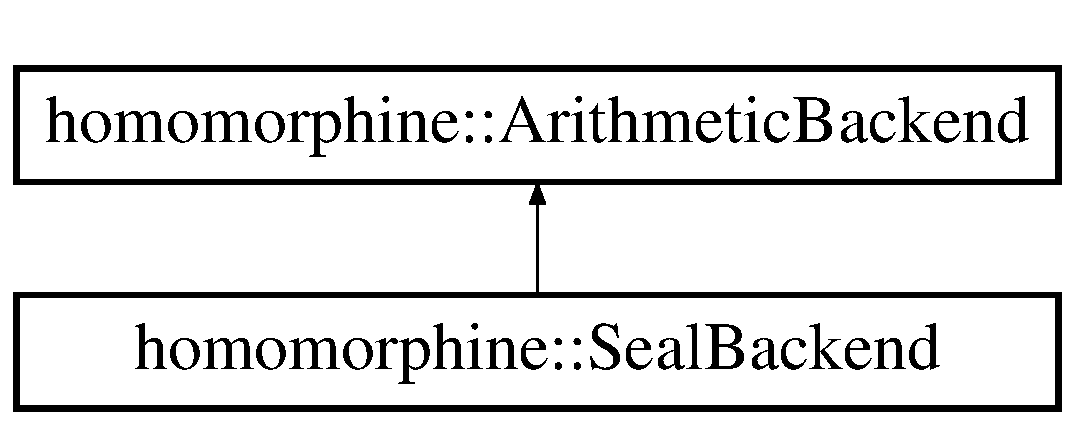
\includegraphics[height=3.000000cm]{classhomomorphine_1_1_seal_backend}
\end{center}
\end{figure}
\subsection*{Public Member Functions}
\begin{DoxyCompactItemize}
\item 
\mbox{\hyperlink{classhomomorphine_1_1_seal_backend_a7224092a19a3472a5143d16b80fb9775}{$\sim$\+Seal\+Backend}} ()
\item 
void \mbox{\hyperlink{classhomomorphine_1_1_seal_backend_a106556100ae5f2e9dadfa9fc64603d94}{init}} ()
\item 
void \mbox{\hyperlink{classhomomorphine_1_1_seal_backend_a46a336bca80c5450a1f3ea1125d0d0e8}{set\+Algorithm}} (string algorithm)
\item 
void \mbox{\hyperlink{classhomomorphine_1_1_seal_backend_aaf2100eb13b4434bc0136ff00578bb8d}{set\+Algorithm}} (Seal\+Algorithm algorithm)
\item 
void \mbox{\hyperlink{classhomomorphine_1_1_seal_backend_a1e2ed46b896d4a5b5d930ec7bcd3207b}{generate\+Keys}} ()
\item 
string \mbox{\hyperlink{classhomomorphine_1_1_seal_backend_aa2dce269303eaa73c62dbfacce66dc1a}{get\+Public\+Key}} ()
\item 
void \mbox{\hyperlink{classhomomorphine_1_1_seal_backend_af09735f0304cc28e6dc967938a4ad277}{write\+Public\+Key\+To\+Stream}} (ostream \&stream)
\item 
string \mbox{\hyperlink{classhomomorphine_1_1_seal_backend_a8ad57a68eb8a02d162ba439046565471}{get\+Secret\+Key}} ()
\item 
void \mbox{\hyperlink{classhomomorphine_1_1_seal_backend_ab3420695131ae4c2a3891917480ddacf}{write\+Secret\+Key\+To\+Stream}} (ostream \&stream)
\item 
pair$<$ string, string $>$ \mbox{\hyperlink{classhomomorphine_1_1_seal_backend_a30358e6405e2d1470468cf55aefb3f4d}{get\+Keys}} ()
\item 
void \mbox{\hyperlink{classhomomorphine_1_1_seal_backend_a6d34008acb06ff1d6743f9163fcd41fb}{set\+Public\+Key}} (string public\+\_\+key)
\item 
void \mbox{\hyperlink{classhomomorphine_1_1_seal_backend_a5bcb7f49667f2a2e095690fdec484b51}{read\+Public\+Key\+From\+Stream}} (istream \&stream)
\item 
void \mbox{\hyperlink{classhomomorphine_1_1_seal_backend_aa9fd3331b2c710e8fdfc3385bbf11eb5}{set\+Secret\+Key}} (string secret\+\_\+key)
\item 
void \mbox{\hyperlink{classhomomorphine_1_1_seal_backend_a5c1607bb712ff2776f4d4ca0c75b3e37}{read\+Secret\+Key\+From\+Stream}} (istream \&stream)
\item 
void \mbox{\hyperlink{classhomomorphine_1_1_seal_backend_a42afcc2823d616edc6be0e3950cf7196}{set\+Keys}} (string public\+\_\+key, string secret\+\_\+key)
\item 
string \mbox{\hyperlink{classhomomorphine_1_1_seal_backend_a0917c586791e74b83f4ca0932e5e4d8e}{get\+Cipher}} ()
\item 
void \mbox{\hyperlink{classhomomorphine_1_1_seal_backend_a2d30b67d872ccd9dc572da2bb08b0635}{write\+Cipher\+To\+Stream}} (ostream \&stream)
\item 
void \mbox{\hyperlink{classhomomorphine_1_1_seal_backend_a866b58e41809d68d4c6ed8c3afb27712}{set\+Cipher}} (string cipher)
\item 
void \mbox{\hyperlink{classhomomorphine_1_1_seal_backend_a2b6704607e71b72122d3820b750f1bee}{read\+Cipher\+From\+Stream}} (istream \&stream)
\item 
void \mbox{\hyperlink{classhomomorphine_1_1_seal_backend_a89ea7aba58ef337476035848c903f08c}{encrypt}} (vector$<$ long $>$ values)
\item 
void \mbox{\hyperlink{classhomomorphine_1_1_seal_backend_aa0815bdb369e3802140efc722a811112}{encrypt}} (long value)
\item 
vector$<$ long $>$ \mbox{\hyperlink{classhomomorphine_1_1_seal_backend_afa5f6cbb10d74c1911fcb88f722a0159}{decrypt\+Values}} ()
\item 
long \mbox{\hyperlink{classhomomorphine_1_1_seal_backend_a0496053defd79b8bd42d4d9c6b4b4ccc}{decrypt}} ()
\item 
void \mbox{\hyperlink{classhomomorphine_1_1_seal_backend_ae868a22dda1eed2246c59aa831707bf1}{add}} (vector$<$ long $>$ values)
\item 
void \mbox{\hyperlink{classhomomorphine_1_1_seal_backend_acbff51d94165f4e578cafaeb965e4367}{add}} (long value)
\item 
void \mbox{\hyperlink{classhomomorphine_1_1_seal_backend_a9064cf9822de85af9120528cef084bea}{negate}} ()
\item 
void \mbox{\hyperlink{classhomomorphine_1_1_seal_backend_ace0bb8cd6a0e4b22f6e3e7ab00ea1197}{multiply}} (vector$<$ long $>$ values)
\item 
void \mbox{\hyperlink{classhomomorphine_1_1_seal_backend_afd8f13068d81c0038b966df4219e8033}{multiply}} (long value)
\end{DoxyCompactItemize}
\subsection*{Additional Inherited Members}


\subsection{Detailed Description}
/brief S\+E\+AL backend

This class is an implementation of the S\+E\+AL backend. 

\subsection{Constructor \& Destructor Documentation}
\mbox{\Hypertarget{classhomomorphine_1_1_seal_backend_a7224092a19a3472a5143d16b80fb9775}\label{classhomomorphine_1_1_seal_backend_a7224092a19a3472a5143d16b80fb9775}} 
\index{homomorphine::SealBackend@{homomorphine::SealBackend}!````~SealBackend@{$\sim$SealBackend}}
\index{````~SealBackend@{$\sim$SealBackend}!homomorphine::SealBackend@{homomorphine::SealBackend}}
\subsubsection{\texorpdfstring{$\sim$SealBackend()}{~SealBackend()}}
{\footnotesize\ttfamily homomorphine\+::\+Seal\+Backend\+::$\sim$\+Seal\+Backend (\begin{DoxyParamCaption}{ }\end{DoxyParamCaption})}

S\+E\+AL backend cleanup 

\subsection{Member Function Documentation}
\mbox{\Hypertarget{classhomomorphine_1_1_seal_backend_ae868a22dda1eed2246c59aa831707bf1}\label{classhomomorphine_1_1_seal_backend_ae868a22dda1eed2246c59aa831707bf1}} 
\index{homomorphine::SealBackend@{homomorphine::SealBackend}!add@{add}}
\index{add@{add}!homomorphine::SealBackend@{homomorphine::SealBackend}}
\subsubsection{\texorpdfstring{add()}{add()}\hspace{0.1cm}{\footnotesize\ttfamily [1/2]}}
{\footnotesize\ttfamily void homomorphine\+::\+Seal\+Backend\+::add (\begin{DoxyParamCaption}\item[{vector$<$ long $>$}]{values }\end{DoxyParamCaption})\hspace{0.3cm}{\ttfamily [virtual]}}

Adds the vector of values to encrypted vector of values


\begin{DoxyParams}{Parameters}
{\em values} & vector of values \\
\hline
\end{DoxyParams}


Implements \mbox{\hyperlink{classhomomorphine_1_1_arithmetic_backend_abf4053e05f07e566e9563a75f516daf6}{homomorphine\+::\+Arithmetic\+Backend}}.

\mbox{\Hypertarget{classhomomorphine_1_1_seal_backend_acbff51d94165f4e578cafaeb965e4367}\label{classhomomorphine_1_1_seal_backend_acbff51d94165f4e578cafaeb965e4367}} 
\index{homomorphine::SealBackend@{homomorphine::SealBackend}!add@{add}}
\index{add@{add}!homomorphine::SealBackend@{homomorphine::SealBackend}}
\subsubsection{\texorpdfstring{add()}{add()}\hspace{0.1cm}{\footnotesize\ttfamily [2/2]}}
{\footnotesize\ttfamily void homomorphine\+::\+Seal\+Backend\+::add (\begin{DoxyParamCaption}\item[{long}]{value }\end{DoxyParamCaption})\hspace{0.3cm}{\ttfamily [virtual]}}

Adds the value to encrypted value


\begin{DoxyParams}{Parameters}
{\em value} & value \\
\hline
\end{DoxyParams}


Implements \mbox{\hyperlink{classhomomorphine_1_1_arithmetic_backend_aa1c88ebc894527a72a9fdbd35ca14204}{homomorphine\+::\+Arithmetic\+Backend}}.

\mbox{\Hypertarget{classhomomorphine_1_1_seal_backend_a0496053defd79b8bd42d4d9c6b4b4ccc}\label{classhomomorphine_1_1_seal_backend_a0496053defd79b8bd42d4d9c6b4b4ccc}} 
\index{homomorphine::SealBackend@{homomorphine::SealBackend}!decrypt@{decrypt}}
\index{decrypt@{decrypt}!homomorphine::SealBackend@{homomorphine::SealBackend}}
\subsubsection{\texorpdfstring{decrypt()}{decrypt()}}
{\footnotesize\ttfamily long homomorphine\+::\+Seal\+Backend\+::decrypt (\begin{DoxyParamCaption}{ }\end{DoxyParamCaption})\hspace{0.3cm}{\ttfamily [virtual]}}

Decrypts the single value using the secret key

\begin{DoxyReturn}{Returns}
decrypted value 
\end{DoxyReturn}


Implements \mbox{\hyperlink{classhomomorphine_1_1_arithmetic_backend_af4aad032c46ce51e608092ac206882bd}{homomorphine\+::\+Arithmetic\+Backend}}.

\mbox{\Hypertarget{classhomomorphine_1_1_seal_backend_afa5f6cbb10d74c1911fcb88f722a0159}\label{classhomomorphine_1_1_seal_backend_afa5f6cbb10d74c1911fcb88f722a0159}} 
\index{homomorphine::SealBackend@{homomorphine::SealBackend}!decryptValues@{decryptValues}}
\index{decryptValues@{decryptValues}!homomorphine::SealBackend@{homomorphine::SealBackend}}
\subsubsection{\texorpdfstring{decryptValues()}{decryptValues()}}
{\footnotesize\ttfamily vector$<$ long $>$ homomorphine\+::\+Seal\+Backend\+::decrypt\+Values (\begin{DoxyParamCaption}{ }\end{DoxyParamCaption})\hspace{0.3cm}{\ttfamily [virtual]}}

Decrypts the vector of values using the secret key

\begin{DoxyReturn}{Returns}
vector of decrypted values 
\end{DoxyReturn}


Implements \mbox{\hyperlink{classhomomorphine_1_1_arithmetic_backend_a2fb1ce64e74c4930b7d364ce3b9cc8fe}{homomorphine\+::\+Arithmetic\+Backend}}.

\mbox{\Hypertarget{classhomomorphine_1_1_seal_backend_a89ea7aba58ef337476035848c903f08c}\label{classhomomorphine_1_1_seal_backend_a89ea7aba58ef337476035848c903f08c}} 
\index{homomorphine::SealBackend@{homomorphine::SealBackend}!encrypt@{encrypt}}
\index{encrypt@{encrypt}!homomorphine::SealBackend@{homomorphine::SealBackend}}
\subsubsection{\texorpdfstring{encrypt()}{encrypt()}\hspace{0.1cm}{\footnotesize\ttfamily [1/2]}}
{\footnotesize\ttfamily void homomorphine\+::\+Seal\+Backend\+::encrypt (\begin{DoxyParamCaption}\item[{vector$<$ long $>$}]{values }\end{DoxyParamCaption})\hspace{0.3cm}{\ttfamily [virtual]}}

Encrypts the vector of values using the public key


\begin{DoxyParams}{Parameters}
{\em values} & vector of values \\
\hline
\end{DoxyParams}
\begin{DoxyReturn}{Returns}
U\+U\+Encoded cipher 
\end{DoxyReturn}


Implements \mbox{\hyperlink{classhomomorphine_1_1_arithmetic_backend_a684c16673191eb5f7c6400f3d34cbcc1}{homomorphine\+::\+Arithmetic\+Backend}}.

\mbox{\Hypertarget{classhomomorphine_1_1_seal_backend_aa0815bdb369e3802140efc722a811112}\label{classhomomorphine_1_1_seal_backend_aa0815bdb369e3802140efc722a811112}} 
\index{homomorphine::SealBackend@{homomorphine::SealBackend}!encrypt@{encrypt}}
\index{encrypt@{encrypt}!homomorphine::SealBackend@{homomorphine::SealBackend}}
\subsubsection{\texorpdfstring{encrypt()}{encrypt()}\hspace{0.1cm}{\footnotesize\ttfamily [2/2]}}
{\footnotesize\ttfamily void homomorphine\+::\+Seal\+Backend\+::encrypt (\begin{DoxyParamCaption}\item[{long}]{value }\end{DoxyParamCaption})\hspace{0.3cm}{\ttfamily [virtual]}}

Encrypts the single value using the public key


\begin{DoxyParams}{Parameters}
{\em value} & value \\
\hline
\end{DoxyParams}
\begin{DoxyReturn}{Returns}
U\+U\+Encoded cipher 
\end{DoxyReturn}


Implements \mbox{\hyperlink{classhomomorphine_1_1_arithmetic_backend_abdf6100f3d87580c942526027823fdb1}{homomorphine\+::\+Arithmetic\+Backend}}.

\mbox{\Hypertarget{classhomomorphine_1_1_seal_backend_a1e2ed46b896d4a5b5d930ec7bcd3207b}\label{classhomomorphine_1_1_seal_backend_a1e2ed46b896d4a5b5d930ec7bcd3207b}} 
\index{homomorphine::SealBackend@{homomorphine::SealBackend}!generateKeys@{generateKeys}}
\index{generateKeys@{generateKeys}!homomorphine::SealBackend@{homomorphine::SealBackend}}
\subsubsection{\texorpdfstring{generateKeys()}{generateKeys()}}
{\footnotesize\ttfamily void homomorphine\+::\+Seal\+Backend\+::generate\+Keys (\begin{DoxyParamCaption}{ }\end{DoxyParamCaption})\hspace{0.3cm}{\ttfamily [virtual]}}

Generates the public/secret key pair 

Implements \mbox{\hyperlink{classhomomorphine_1_1_arithmetic_backend_a5faa0089b80be5629d4a0a7a02fe3568}{homomorphine\+::\+Arithmetic\+Backend}}.

\mbox{\Hypertarget{classhomomorphine_1_1_seal_backend_a0917c586791e74b83f4ca0932e5e4d8e}\label{classhomomorphine_1_1_seal_backend_a0917c586791e74b83f4ca0932e5e4d8e}} 
\index{homomorphine::SealBackend@{homomorphine::SealBackend}!getCipher@{getCipher}}
\index{getCipher@{getCipher}!homomorphine::SealBackend@{homomorphine::SealBackend}}
\subsubsection{\texorpdfstring{getCipher()}{getCipher()}}
{\footnotesize\ttfamily string homomorphine\+::\+Seal\+Backend\+::get\+Cipher (\begin{DoxyParamCaption}{ }\end{DoxyParamCaption})\hspace{0.3cm}{\ttfamily [virtual]}}

Returns the U\+U\+Encoded cipher containing ecrypted value, or vector of values

\begin{DoxyReturn}{Returns}
U\+U\+Encoded cipher 
\end{DoxyReturn}


Implements \mbox{\hyperlink{classhomomorphine_1_1_arithmetic_backend_acf38918fb556703ccb12b63dc73b15ed}{homomorphine\+::\+Arithmetic\+Backend}}.

\mbox{\Hypertarget{classhomomorphine_1_1_seal_backend_a30358e6405e2d1470468cf55aefb3f4d}\label{classhomomorphine_1_1_seal_backend_a30358e6405e2d1470468cf55aefb3f4d}} 
\index{homomorphine::SealBackend@{homomorphine::SealBackend}!getKeys@{getKeys}}
\index{getKeys@{getKeys}!homomorphine::SealBackend@{homomorphine::SealBackend}}
\subsubsection{\texorpdfstring{getKeys()}{getKeys()}}
{\footnotesize\ttfamily pair$<$ string, string $>$ homomorphine\+::\+Seal\+Backend\+::get\+Keys (\begin{DoxyParamCaption}{ }\end{DoxyParamCaption})\hspace{0.3cm}{\ttfamily [virtual]}}

Returns the pair of U\+U\+Encoded public and secret keys

\begin{DoxyReturn}{Returns}
pair of public and secret keys 
\end{DoxyReturn}


Implements \mbox{\hyperlink{classhomomorphine_1_1_arithmetic_backend_a71bb86054685708001c636e3085d578c}{homomorphine\+::\+Arithmetic\+Backend}}.

\mbox{\Hypertarget{classhomomorphine_1_1_seal_backend_aa2dce269303eaa73c62dbfacce66dc1a}\label{classhomomorphine_1_1_seal_backend_aa2dce269303eaa73c62dbfacce66dc1a}} 
\index{homomorphine::SealBackend@{homomorphine::SealBackend}!getPublicKey@{getPublicKey}}
\index{getPublicKey@{getPublicKey}!homomorphine::SealBackend@{homomorphine::SealBackend}}
\subsubsection{\texorpdfstring{getPublicKey()}{getPublicKey()}}
{\footnotesize\ttfamily string homomorphine\+::\+Seal\+Backend\+::get\+Public\+Key (\begin{DoxyParamCaption}{ }\end{DoxyParamCaption})\hspace{0.3cm}{\ttfamily [virtual]}}

Returns the U\+U\+Encoded public key

\begin{DoxyReturn}{Returns}
public key 
\end{DoxyReturn}


Implements \mbox{\hyperlink{classhomomorphine_1_1_arithmetic_backend_a26f31fc0c76cf58636972f68142b9a06}{homomorphine\+::\+Arithmetic\+Backend}}.

\mbox{\Hypertarget{classhomomorphine_1_1_seal_backend_a8ad57a68eb8a02d162ba439046565471}\label{classhomomorphine_1_1_seal_backend_a8ad57a68eb8a02d162ba439046565471}} 
\index{homomorphine::SealBackend@{homomorphine::SealBackend}!getSecretKey@{getSecretKey}}
\index{getSecretKey@{getSecretKey}!homomorphine::SealBackend@{homomorphine::SealBackend}}
\subsubsection{\texorpdfstring{getSecretKey()}{getSecretKey()}}
{\footnotesize\ttfamily string homomorphine\+::\+Seal\+Backend\+::get\+Secret\+Key (\begin{DoxyParamCaption}{ }\end{DoxyParamCaption})\hspace{0.3cm}{\ttfamily [virtual]}}

Returns the U\+U\+Encoded secret key

\begin{DoxyReturn}{Returns}
secret key 
\end{DoxyReturn}


Implements \mbox{\hyperlink{classhomomorphine_1_1_arithmetic_backend_a679abf60fea83922f7972498c4500252}{homomorphine\+::\+Arithmetic\+Backend}}.

\mbox{\Hypertarget{classhomomorphine_1_1_seal_backend_a106556100ae5f2e9dadfa9fc64603d94}\label{classhomomorphine_1_1_seal_backend_a106556100ae5f2e9dadfa9fc64603d94}} 
\index{homomorphine::SealBackend@{homomorphine::SealBackend}!init@{init}}
\index{init@{init}!homomorphine::SealBackend@{homomorphine::SealBackend}}
\subsubsection{\texorpdfstring{init()}{init()}}
{\footnotesize\ttfamily void homomorphine\+::\+Seal\+Backend\+::init (\begin{DoxyParamCaption}{ }\end{DoxyParamCaption})\hspace{0.3cm}{\ttfamily [virtual]}}

Initializes the S\+E\+AL backend 

Implements \mbox{\hyperlink{classhomomorphine_1_1_arithmetic_backend_a2654ee62a6cf2f16fd41c834a26b0006}{homomorphine\+::\+Arithmetic\+Backend}}.

\mbox{\Hypertarget{classhomomorphine_1_1_seal_backend_ace0bb8cd6a0e4b22f6e3e7ab00ea1197}\label{classhomomorphine_1_1_seal_backend_ace0bb8cd6a0e4b22f6e3e7ab00ea1197}} 
\index{homomorphine::SealBackend@{homomorphine::SealBackend}!multiply@{multiply}}
\index{multiply@{multiply}!homomorphine::SealBackend@{homomorphine::SealBackend}}
\subsubsection{\texorpdfstring{multiply()}{multiply()}\hspace{0.1cm}{\footnotesize\ttfamily [1/2]}}
{\footnotesize\ttfamily void homomorphine\+::\+Seal\+Backend\+::multiply (\begin{DoxyParamCaption}\item[{vector$<$ long $>$}]{values }\end{DoxyParamCaption})\hspace{0.3cm}{\ttfamily [virtual]}}

Multiplies the vector of values with the encrypted vector of values


\begin{DoxyParams}{Parameters}
{\em values} & vector of values \\
\hline
\end{DoxyParams}


Implements \mbox{\hyperlink{classhomomorphine_1_1_arithmetic_backend_a80f2424d26fcfad4803f6a0e5a9cdd2d}{homomorphine\+::\+Arithmetic\+Backend}}.

\mbox{\Hypertarget{classhomomorphine_1_1_seal_backend_afd8f13068d81c0038b966df4219e8033}\label{classhomomorphine_1_1_seal_backend_afd8f13068d81c0038b966df4219e8033}} 
\index{homomorphine::SealBackend@{homomorphine::SealBackend}!multiply@{multiply}}
\index{multiply@{multiply}!homomorphine::SealBackend@{homomorphine::SealBackend}}
\subsubsection{\texorpdfstring{multiply()}{multiply()}\hspace{0.1cm}{\footnotesize\ttfamily [2/2]}}
{\footnotesize\ttfamily void homomorphine\+::\+Seal\+Backend\+::multiply (\begin{DoxyParamCaption}\item[{long}]{value }\end{DoxyParamCaption})\hspace{0.3cm}{\ttfamily [virtual]}}

Multiplies the value with the encrypted value


\begin{DoxyParams}{Parameters}
{\em value} & value \\
\hline
\end{DoxyParams}


Implements \mbox{\hyperlink{classhomomorphine_1_1_arithmetic_backend_a22f4c598c5a3987ef6efe5925f4c5b81}{homomorphine\+::\+Arithmetic\+Backend}}.

\mbox{\Hypertarget{classhomomorphine_1_1_seal_backend_a9064cf9822de85af9120528cef084bea}\label{classhomomorphine_1_1_seal_backend_a9064cf9822de85af9120528cef084bea}} 
\index{homomorphine::SealBackend@{homomorphine::SealBackend}!negate@{negate}}
\index{negate@{negate}!homomorphine::SealBackend@{homomorphine::SealBackend}}
\subsubsection{\texorpdfstring{negate()}{negate()}}
{\footnotesize\ttfamily void homomorphine\+::\+Seal\+Backend\+::negate (\begin{DoxyParamCaption}{ }\end{DoxyParamCaption})\hspace{0.3cm}{\ttfamily [virtual]}}

Negates a single encrypted value, or a vector of encrypted values 

Implements \mbox{\hyperlink{classhomomorphine_1_1_arithmetic_backend_ad27913060534c42b5812a1e4cf21475f}{homomorphine\+::\+Arithmetic\+Backend}}.

\mbox{\Hypertarget{classhomomorphine_1_1_seal_backend_a2b6704607e71b72122d3820b750f1bee}\label{classhomomorphine_1_1_seal_backend_a2b6704607e71b72122d3820b750f1bee}} 
\index{homomorphine::SealBackend@{homomorphine::SealBackend}!readCipherFromStream@{readCipherFromStream}}
\index{readCipherFromStream@{readCipherFromStream}!homomorphine::SealBackend@{homomorphine::SealBackend}}
\subsubsection{\texorpdfstring{readCipherFromStream()}{readCipherFromStream()}}
{\footnotesize\ttfamily void homomorphine\+::\+Seal\+Backend\+::read\+Cipher\+From\+Stream (\begin{DoxyParamCaption}\item[{istream \&}]{stream }\end{DoxyParamCaption})\hspace{0.3cm}{\ttfamily [virtual]}}

Reads the cipher from input stream


\begin{DoxyParams}{Parameters}
{\em stream} & cipher stream \\
\hline
\end{DoxyParams}


Implements \mbox{\hyperlink{classhomomorphine_1_1_arithmetic_backend_ac8fe4568424c616b653a955b172c480b}{homomorphine\+::\+Arithmetic\+Backend}}.

\mbox{\Hypertarget{classhomomorphine_1_1_seal_backend_a5bcb7f49667f2a2e095690fdec484b51}\label{classhomomorphine_1_1_seal_backend_a5bcb7f49667f2a2e095690fdec484b51}} 
\index{homomorphine::SealBackend@{homomorphine::SealBackend}!readPublicKeyFromStream@{readPublicKeyFromStream}}
\index{readPublicKeyFromStream@{readPublicKeyFromStream}!homomorphine::SealBackend@{homomorphine::SealBackend}}
\subsubsection{\texorpdfstring{readPublicKeyFromStream()}{readPublicKeyFromStream()}}
{\footnotesize\ttfamily void homomorphine\+::\+Seal\+Backend\+::read\+Public\+Key\+From\+Stream (\begin{DoxyParamCaption}\item[{istream \&}]{stream }\end{DoxyParamCaption})\hspace{0.3cm}{\ttfamily [virtual]}}

Sets the public key from stream


\begin{DoxyParams}{Parameters}
{\em stream} & public key binary stream \\
\hline
\end{DoxyParams}


Implements \mbox{\hyperlink{classhomomorphine_1_1_arithmetic_backend_aab5aac202ce0911e99e8adce7ffb707a}{homomorphine\+::\+Arithmetic\+Backend}}.

\mbox{\Hypertarget{classhomomorphine_1_1_seal_backend_a5c1607bb712ff2776f4d4ca0c75b3e37}\label{classhomomorphine_1_1_seal_backend_a5c1607bb712ff2776f4d4ca0c75b3e37}} 
\index{homomorphine::SealBackend@{homomorphine::SealBackend}!readSecretKeyFromStream@{readSecretKeyFromStream}}
\index{readSecretKeyFromStream@{readSecretKeyFromStream}!homomorphine::SealBackend@{homomorphine::SealBackend}}
\subsubsection{\texorpdfstring{readSecretKeyFromStream()}{readSecretKeyFromStream()}}
{\footnotesize\ttfamily void homomorphine\+::\+Seal\+Backend\+::read\+Secret\+Key\+From\+Stream (\begin{DoxyParamCaption}\item[{istream \&}]{stream }\end{DoxyParamCaption})\hspace{0.3cm}{\ttfamily [virtual]}}

Sets the secret key from stream


\begin{DoxyParams}{Parameters}
{\em stream} & secret key binary stream \\
\hline
\end{DoxyParams}


Implements \mbox{\hyperlink{classhomomorphine_1_1_arithmetic_backend_a69b65cd979de00a9afa0c38c3b4329b0}{homomorphine\+::\+Arithmetic\+Backend}}.

\mbox{\Hypertarget{classhomomorphine_1_1_seal_backend_a46a336bca80c5450a1f3ea1125d0d0e8}\label{classhomomorphine_1_1_seal_backend_a46a336bca80c5450a1f3ea1125d0d0e8}} 
\index{homomorphine::SealBackend@{homomorphine::SealBackend}!setAlgorithm@{setAlgorithm}}
\index{setAlgorithm@{setAlgorithm}!homomorphine::SealBackend@{homomorphine::SealBackend}}
\subsubsection{\texorpdfstring{setAlgorithm()}{setAlgorithm()}\hspace{0.1cm}{\footnotesize\ttfamily [1/2]}}
{\footnotesize\ttfamily void homomorphine\+::\+Seal\+Backend\+::set\+Algorithm (\begin{DoxyParamCaption}\item[{string}]{algorithm }\end{DoxyParamCaption})\hspace{0.3cm}{\ttfamily [virtual]}}

Sets the specific S\+E\+AL algorithm implementation that backend provides (currently, B\+FV and C\+K\+KS)


\begin{DoxyParams}{Parameters}
{\em algorithm} & homomorphic encryption algorithm \\
\hline
\end{DoxyParams}


Implements \mbox{\hyperlink{classhomomorphine_1_1_arithmetic_backend_ac53135f4f66a2f7a33d3c6e6d465b86f}{homomorphine\+::\+Arithmetic\+Backend}}.

\mbox{\Hypertarget{classhomomorphine_1_1_seal_backend_aaf2100eb13b4434bc0136ff00578bb8d}\label{classhomomorphine_1_1_seal_backend_aaf2100eb13b4434bc0136ff00578bb8d}} 
\index{homomorphine::SealBackend@{homomorphine::SealBackend}!setAlgorithm@{setAlgorithm}}
\index{setAlgorithm@{setAlgorithm}!homomorphine::SealBackend@{homomorphine::SealBackend}}
\subsubsection{\texorpdfstring{setAlgorithm()}{setAlgorithm()}\hspace{0.1cm}{\footnotesize\ttfamily [2/2]}}
{\footnotesize\ttfamily void homomorphine\+::\+Seal\+Backend\+::set\+Algorithm (\begin{DoxyParamCaption}\item[{Seal\+Algorithm}]{algorithm }\end{DoxyParamCaption})}

Sets the specific S\+E\+AL algorithm implementation that backend provides using the name of algorithm


\begin{DoxyParams}{Parameters}
{\em algorithm} & homomorphic encryption algorithm \\
\hline
\end{DoxyParams}
\mbox{\Hypertarget{classhomomorphine_1_1_seal_backend_a866b58e41809d68d4c6ed8c3afb27712}\label{classhomomorphine_1_1_seal_backend_a866b58e41809d68d4c6ed8c3afb27712}} 
\index{homomorphine::SealBackend@{homomorphine::SealBackend}!setCipher@{setCipher}}
\index{setCipher@{setCipher}!homomorphine::SealBackend@{homomorphine::SealBackend}}
\subsubsection{\texorpdfstring{setCipher()}{setCipher()}}
{\footnotesize\ttfamily void homomorphine\+::\+Seal\+Backend\+::set\+Cipher (\begin{DoxyParamCaption}\item[{string}]{cipher }\end{DoxyParamCaption})\hspace{0.3cm}{\ttfamily [virtual]}}

Sets the U\+U\+Encoded cipher containing ecrypted value, or vector of values


\begin{DoxyParams}{Parameters}
{\em cipher} & U\+U\+Encoded cipher \\
\hline
\end{DoxyParams}


Implements \mbox{\hyperlink{classhomomorphine_1_1_arithmetic_backend_af9b2d3b33a03d79facdf113c9560fc0b}{homomorphine\+::\+Arithmetic\+Backend}}.

\mbox{\Hypertarget{classhomomorphine_1_1_seal_backend_a42afcc2823d616edc6be0e3950cf7196}\label{classhomomorphine_1_1_seal_backend_a42afcc2823d616edc6be0e3950cf7196}} 
\index{homomorphine::SealBackend@{homomorphine::SealBackend}!setKeys@{setKeys}}
\index{setKeys@{setKeys}!homomorphine::SealBackend@{homomorphine::SealBackend}}
\subsubsection{\texorpdfstring{setKeys()}{setKeys()}}
{\footnotesize\ttfamily void homomorphine\+::\+Seal\+Backend\+::set\+Keys (\begin{DoxyParamCaption}\item[{string}]{public\+\_\+key,  }\item[{string}]{secret\+\_\+key }\end{DoxyParamCaption})\hspace{0.3cm}{\ttfamily [virtual]}}

Sets the both public and secret keys


\begin{DoxyParams}{Parameters}
{\em public\+\_\+key} & U\+U\+Encoded public key \\
\hline
{\em secret\+\_\+key} & U\+U\+Encoded secret key \\
\hline
\end{DoxyParams}


Implements \mbox{\hyperlink{classhomomorphine_1_1_arithmetic_backend_ac78f4b42dce3dce23edd81dba60b16c8}{homomorphine\+::\+Arithmetic\+Backend}}.

\mbox{\Hypertarget{classhomomorphine_1_1_seal_backend_a6d34008acb06ff1d6743f9163fcd41fb}\label{classhomomorphine_1_1_seal_backend_a6d34008acb06ff1d6743f9163fcd41fb}} 
\index{homomorphine::SealBackend@{homomorphine::SealBackend}!setPublicKey@{setPublicKey}}
\index{setPublicKey@{setPublicKey}!homomorphine::SealBackend@{homomorphine::SealBackend}}
\subsubsection{\texorpdfstring{setPublicKey()}{setPublicKey()}}
{\footnotesize\ttfamily void homomorphine\+::\+Seal\+Backend\+::set\+Public\+Key (\begin{DoxyParamCaption}\item[{string}]{public\+\_\+key }\end{DoxyParamCaption})\hspace{0.3cm}{\ttfamily [virtual]}}

Sets the public key


\begin{DoxyParams}{Parameters}
{\em public\+\_\+key} & U\+U\+Encoded public key \\
\hline
\end{DoxyParams}


Implements \mbox{\hyperlink{classhomomorphine_1_1_arithmetic_backend_af2dd2c37ed1fcd56b58baa6cb3f14e8b}{homomorphine\+::\+Arithmetic\+Backend}}.

\mbox{\Hypertarget{classhomomorphine_1_1_seal_backend_aa9fd3331b2c710e8fdfc3385bbf11eb5}\label{classhomomorphine_1_1_seal_backend_aa9fd3331b2c710e8fdfc3385bbf11eb5}} 
\index{homomorphine::SealBackend@{homomorphine::SealBackend}!setSecretKey@{setSecretKey}}
\index{setSecretKey@{setSecretKey}!homomorphine::SealBackend@{homomorphine::SealBackend}}
\subsubsection{\texorpdfstring{setSecretKey()}{setSecretKey()}}
{\footnotesize\ttfamily void homomorphine\+::\+Seal\+Backend\+::set\+Secret\+Key (\begin{DoxyParamCaption}\item[{string}]{secret\+\_\+key }\end{DoxyParamCaption})\hspace{0.3cm}{\ttfamily [virtual]}}

Sets the secret key


\begin{DoxyParams}{Parameters}
{\em secret\+\_\+key} & U\+U\+Encoded secret key \\
\hline
\end{DoxyParams}


Implements \mbox{\hyperlink{classhomomorphine_1_1_arithmetic_backend_a0bb3c2728df4662c6472d4d43215410f}{homomorphine\+::\+Arithmetic\+Backend}}.

\mbox{\Hypertarget{classhomomorphine_1_1_seal_backend_a2d30b67d872ccd9dc572da2bb08b0635}\label{classhomomorphine_1_1_seal_backend_a2d30b67d872ccd9dc572da2bb08b0635}} 
\index{homomorphine::SealBackend@{homomorphine::SealBackend}!writeCipherToStream@{writeCipherToStream}}
\index{writeCipherToStream@{writeCipherToStream}!homomorphine::SealBackend@{homomorphine::SealBackend}}
\subsubsection{\texorpdfstring{writeCipherToStream()}{writeCipherToStream()}}
{\footnotesize\ttfamily void homomorphine\+::\+Seal\+Backend\+::write\+Cipher\+To\+Stream (\begin{DoxyParamCaption}\item[{ostream \&}]{stream }\end{DoxyParamCaption})\hspace{0.3cm}{\ttfamily [virtual]}}

Writes the cipher to output stream


\begin{DoxyParams}{Parameters}
{\em stream} & output stream \\
\hline
\end{DoxyParams}


Implements \mbox{\hyperlink{classhomomorphine_1_1_arithmetic_backend_a659d4f63a1020d942d561b7fa5e9eddf}{homomorphine\+::\+Arithmetic\+Backend}}.

\mbox{\Hypertarget{classhomomorphine_1_1_seal_backend_af09735f0304cc28e6dc967938a4ad277}\label{classhomomorphine_1_1_seal_backend_af09735f0304cc28e6dc967938a4ad277}} 
\index{homomorphine::SealBackend@{homomorphine::SealBackend}!writePublicKeyToStream@{writePublicKeyToStream}}
\index{writePublicKeyToStream@{writePublicKeyToStream}!homomorphine::SealBackend@{homomorphine::SealBackend}}
\subsubsection{\texorpdfstring{writePublicKeyToStream()}{writePublicKeyToStream()}}
{\footnotesize\ttfamily void homomorphine\+::\+Seal\+Backend\+::write\+Public\+Key\+To\+Stream (\begin{DoxyParamCaption}\item[{ostream \&}]{stream }\end{DoxyParamCaption})\hspace{0.3cm}{\ttfamily [virtual]}}

Writes the public key to a stream


\begin{DoxyParams}{Parameters}
{\em stream} & public key stream \\
\hline
\end{DoxyParams}


Implements \mbox{\hyperlink{classhomomorphine_1_1_arithmetic_backend_a2552b81a08e286969a0ff44428d59af4}{homomorphine\+::\+Arithmetic\+Backend}}.

\mbox{\Hypertarget{classhomomorphine_1_1_seal_backend_ab3420695131ae4c2a3891917480ddacf}\label{classhomomorphine_1_1_seal_backend_ab3420695131ae4c2a3891917480ddacf}} 
\index{homomorphine::SealBackend@{homomorphine::SealBackend}!writeSecretKeyToStream@{writeSecretKeyToStream}}
\index{writeSecretKeyToStream@{writeSecretKeyToStream}!homomorphine::SealBackend@{homomorphine::SealBackend}}
\subsubsection{\texorpdfstring{writeSecretKeyToStream()}{writeSecretKeyToStream()}}
{\footnotesize\ttfamily void homomorphine\+::\+Seal\+Backend\+::write\+Secret\+Key\+To\+Stream (\begin{DoxyParamCaption}\item[{ostream \&}]{stream }\end{DoxyParamCaption})\hspace{0.3cm}{\ttfamily [virtual]}}

Writes the secret key to a stream


\begin{DoxyParams}{Parameters}
{\em stream} & secret key stream \\
\hline
\end{DoxyParams}


Implements \mbox{\hyperlink{classhomomorphine_1_1_arithmetic_backend_ad88c797bbb2073ed3af460e568725c3f}{homomorphine\+::\+Arithmetic\+Backend}}.



The documentation for this class was generated from the following files\+:\begin{DoxyCompactItemize}
\item 
src/seal\+\_\+backend.\+hpp\item 
src/seal\+\_\+backend.\+cpp\end{DoxyCompactItemize}

\hypertarget{classhomomorphine_1_1_server}{}\section{homomorphine\+::Server Class Reference}
\label{classhomomorphine_1_1_server}\index{homomorphine::Server@{homomorphine::Server}}


{\ttfamily \#include $<$server.\+hpp$>$}

\subsection*{Public Member Functions}
\begin{DoxyCompactItemize}
\item 
void \mbox{\hyperlink{classhomomorphine_1_1_server_a0fcfa773dc495f0741387cdb11f95ea0}{init}} (\mbox{\hyperlink{classhomomorphine_1_1_config}{Config}} \&config)
\item 
void \mbox{\hyperlink{classhomomorphine_1_1_server_a02ae1a9f2334652a64a498e6a6efc4b1}{run}} ()
\item 
void \mbox{\hyperlink{classhomomorphine_1_1_server_a5655dfcc0a213e6bf1f8d35dbadebf4d}{stop}} ()
\end{DoxyCompactItemize}


\subsection{Detailed Description}
/brief Homomorphine R\+E\+S\+T\+Ful service

This class implements a R\+E\+S\+T\+Ful service that can be used to test various aspects of Homomorphine functionalities. This service is not intended for a production usage. 

\subsection{Member Function Documentation}
\mbox{\Hypertarget{classhomomorphine_1_1_server_a0fcfa773dc495f0741387cdb11f95ea0}\label{classhomomorphine_1_1_server_a0fcfa773dc495f0741387cdb11f95ea0}} 
\index{homomorphine::Server@{homomorphine::Server}!init@{init}}
\index{init@{init}!homomorphine::Server@{homomorphine::Server}}
\subsubsection{\texorpdfstring{init()}{init()}}
{\footnotesize\ttfamily void homomorphine\+::\+Server\+::init (\begin{DoxyParamCaption}\item[{\mbox{\hyperlink{classhomomorphine_1_1_config}{Config}} \&}]{config }\end{DoxyParamCaption})}

Initialization of Homomorphine R\+E\+S\+T\+Ful service


\begin{DoxyParams}{Parameters}
{\em config} & service configuration \\
\hline
\end{DoxyParams}
\mbox{\Hypertarget{classhomomorphine_1_1_server_a02ae1a9f2334652a64a498e6a6efc4b1}\label{classhomomorphine_1_1_server_a02ae1a9f2334652a64a498e6a6efc4b1}} 
\index{homomorphine::Server@{homomorphine::Server}!run@{run}}
\index{run@{run}!homomorphine::Server@{homomorphine::Server}}
\subsubsection{\texorpdfstring{run()}{run()}}
{\footnotesize\ttfamily void homomorphine\+::\+Server\+::run (\begin{DoxyParamCaption}{ }\end{DoxyParamCaption})}

Start R\+E\+S\+T\+Ful service \mbox{\Hypertarget{classhomomorphine_1_1_server_a5655dfcc0a213e6bf1f8d35dbadebf4d}\label{classhomomorphine_1_1_server_a5655dfcc0a213e6bf1f8d35dbadebf4d}} 
\index{homomorphine::Server@{homomorphine::Server}!stop@{stop}}
\index{stop@{stop}!homomorphine::Server@{homomorphine::Server}}
\subsubsection{\texorpdfstring{stop()}{stop()}}
{\footnotesize\ttfamily void homomorphine\+::\+Server\+::stop (\begin{DoxyParamCaption}{ }\end{DoxyParamCaption})}

Stop R\+E\+S\+T\+Ful service 

The documentation for this class was generated from the following files\+:\begin{DoxyCompactItemize}
\item 
src/server.\+hpp\item 
src/server.\+cpp\end{DoxyCompactItemize}

\input{classhomomorphine_1_1_t_f_h_e_backend}
\hypertarget{classhomomorphine_1_1_util}{}\section{homomorphine\+::Util Class Reference}
\label{classhomomorphine_1_1_util}\index{homomorphine::Util@{homomorphine::Util}}


{\ttfamily \#include $<$util.\+hpp$>$}

\subsection*{Static Public Member Functions}
\begin{DoxyCompactItemize}
\item 
static const string \mbox{\hyperlink{classhomomorphine_1_1_util_a26f29995aa48f4374993ec4afeca2ac8}{uuencode\+Stream}} (stringstream \&string\+\_\+stream)
\item 
static const void \mbox{\hyperlink{classhomomorphine_1_1_util_aba5af6d7356aca8c70ae4fb1e5d36b70}{uudecode\+String}} (string content, stringstream \&string\+\_\+stream)
\item 
static const vector$<$ int $>$ \mbox{\hyperlink{classhomomorphine_1_1_util_a2dcf1d83028f3d47ba49b80696fefef7}{get\+Random\+Vector}} (int \&size)
\item 
static const long \mbox{\hyperlink{classhomomorphine_1_1_util_acf2321afce14e9c20ca572159592e0e2}{get\+Stream\+Size}} (istream \&stream)
\item 
static const \mbox{\hyperlink{structbyte__array__t}{bytes}} \mbox{\hyperlink{classhomomorphine_1_1_util_af81e87e9babd7ab4cd37cd3d1725c5b5}{copy\+Stream\+To\+Bytes}} (istream \&stream)
\end{DoxyCompactItemize}


\subsection{Detailed Description}
/brief Utility class

This class provides a various utility functions. At this moment it supports U\+U\+Encoding/\+U\+U\+Decoding of the binary string streams used to serialize various binary objects for external usage and standardization of the interface. 

\subsection{Member Function Documentation}
\mbox{\Hypertarget{classhomomorphine_1_1_util_af81e87e9babd7ab4cd37cd3d1725c5b5}\label{classhomomorphine_1_1_util_af81e87e9babd7ab4cd37cd3d1725c5b5}} 
\index{homomorphine::Util@{homomorphine::Util}!copyStreamToBytes@{copyStreamToBytes}}
\index{copyStreamToBytes@{copyStreamToBytes}!homomorphine::Util@{homomorphine::Util}}
\subsubsection{\texorpdfstring{copyStreamToBytes()}{copyStreamToBytes()}}
{\footnotesize\ttfamily const \mbox{\hyperlink{structbyte__array__t}{bytes}} homomorphine\+::\+Util\+::copy\+Stream\+To\+Bytes (\begin{DoxyParamCaption}\item[{istream \&}]{stream }\end{DoxyParamCaption})\hspace{0.3cm}{\ttfamily [static]}}

Loads the content of stream to bytes structure -\/ required for handling byte streams that can\textquotesingle{}t be simply copied into strings, or char arrays without additional encoding


\begin{DoxyParams}{Parameters}
{\em stream} & input stream \\
\hline
\end{DoxyParams}
\begin{DoxyReturn}{Returns}
bytes P\+OD structure 
\end{DoxyReturn}
\mbox{\Hypertarget{classhomomorphine_1_1_util_a2dcf1d83028f3d47ba49b80696fefef7}\label{classhomomorphine_1_1_util_a2dcf1d83028f3d47ba49b80696fefef7}} 
\index{homomorphine::Util@{homomorphine::Util}!getRandomVector@{getRandomVector}}
\index{getRandomVector@{getRandomVector}!homomorphine::Util@{homomorphine::Util}}
\subsubsection{\texorpdfstring{getRandomVector()}{getRandomVector()}}
{\footnotesize\ttfamily const vector$<$ int $>$ homomorphine\+::\+Util\+::get\+Random\+Vector (\begin{DoxyParamCaption}\item[{int \&}]{size }\end{DoxyParamCaption})\hspace{0.3cm}{\ttfamily [static]}}

Generates a vector of random values


\begin{DoxyParams}{Parameters}
{\em size} & size of vector \\
\hline
\end{DoxyParams}
\begin{DoxyReturn}{Returns}
vector of random numbers 
\end{DoxyReturn}
\mbox{\Hypertarget{classhomomorphine_1_1_util_acf2321afce14e9c20ca572159592e0e2}\label{classhomomorphine_1_1_util_acf2321afce14e9c20ca572159592e0e2}} 
\index{homomorphine::Util@{homomorphine::Util}!getStreamSize@{getStreamSize}}
\index{getStreamSize@{getStreamSize}!homomorphine::Util@{homomorphine::Util}}
\subsubsection{\texorpdfstring{getStreamSize()}{getStreamSize()}}
{\footnotesize\ttfamily const long homomorphine\+::\+Util\+::get\+Stream\+Size (\begin{DoxyParamCaption}\item[{istream \&}]{stream }\end{DoxyParamCaption})\hspace{0.3cm}{\ttfamily [static]}}

Returns total size of input stream in bytes


\begin{DoxyParams}{Parameters}
{\em stream} & input stream size \\
\hline
\end{DoxyParams}
\begin{DoxyReturn}{Returns}
stream size in bytes 
\end{DoxyReturn}
\mbox{\Hypertarget{classhomomorphine_1_1_util_aba5af6d7356aca8c70ae4fb1e5d36b70}\label{classhomomorphine_1_1_util_aba5af6d7356aca8c70ae4fb1e5d36b70}} 
\index{homomorphine::Util@{homomorphine::Util}!uudecodeString@{uudecodeString}}
\index{uudecodeString@{uudecodeString}!homomorphine::Util@{homomorphine::Util}}
\subsubsection{\texorpdfstring{uudecodeString()}{uudecodeString()}}
{\footnotesize\ttfamily const void homomorphine\+::\+Util\+::uudecode\+String (\begin{DoxyParamCaption}\item[{string}]{content,  }\item[{stringstream \&}]{string\+\_\+stream }\end{DoxyParamCaption})\hspace{0.3cm}{\ttfamily [static]}}

Decodes U\+U\+Encoded string to a binary string stream


\begin{DoxyParams}{Parameters}
{\em content} & U\+U\+E\+Ncoded string \\
\hline
{\em string\+\_\+stream} & stream containing a decoded stream \\
\hline
\end{DoxyParams}
\mbox{\Hypertarget{classhomomorphine_1_1_util_a26f29995aa48f4374993ec4afeca2ac8}\label{classhomomorphine_1_1_util_a26f29995aa48f4374993ec4afeca2ac8}} 
\index{homomorphine::Util@{homomorphine::Util}!uuencodeStream@{uuencodeStream}}
\index{uuencodeStream@{uuencodeStream}!homomorphine::Util@{homomorphine::Util}}
\subsubsection{\texorpdfstring{uuencodeStream()}{uuencodeStream()}}
{\footnotesize\ttfamily const string homomorphine\+::\+Util\+::uuencode\+Stream (\begin{DoxyParamCaption}\item[{stringstream \&}]{string\+\_\+stream }\end{DoxyParamCaption})\hspace{0.3cm}{\ttfamily [static]}}

Encodes the binary string stream to string


\begin{DoxyParams}{Parameters}
{\em string\+\_\+stream} & string stream to be U\+U\+Encoded \\
\hline
\end{DoxyParams}
\begin{DoxyReturn}{Returns}
U\+U\+Encoded string 
\end{DoxyReturn}


The documentation for this class was generated from the following files\+:\begin{DoxyCompactItemize}
\item 
src/util.\+hpp\item 
src/util.\+cpp\end{DoxyCompactItemize}

%--- End generated contents ---

% Index
\backmatter
\newpage
\phantomsection
\clearemptydoublepage
\addcontentsline{toc}{chapter}{Index}
\printindex

\end{document}
